% Options for packages loaded elsewhere
\PassOptionsToPackage{unicode}{hyperref}
\PassOptionsToPackage{hyphens}{url}
%
\documentclass[
  man,floatsintext]{apa6}
\usepackage{amsmath,amssymb}
\usepackage{lmodern}
\usepackage{iftex}
\ifPDFTeX
  \usepackage[T1]{fontenc}
  \usepackage[utf8]{inputenc}
  \usepackage{textcomp} % provide euro and other symbols
\else % if luatex or xetex
  \usepackage{unicode-math}
  \defaultfontfeatures{Scale=MatchLowercase}
  \defaultfontfeatures[\rmfamily]{Ligatures=TeX,Scale=1}
\fi
% Use upquote if available, for straight quotes in verbatim environments
\IfFileExists{upquote.sty}{\usepackage{upquote}}{}
\IfFileExists{microtype.sty}{% use microtype if available
  \usepackage[]{microtype}
  \UseMicrotypeSet[protrusion]{basicmath} % disable protrusion for tt fonts
}{}
\makeatletter
\@ifundefined{KOMAClassName}{% if non-KOMA class
  \IfFileExists{parskip.sty}{%
    \usepackage{parskip}
  }{% else
    \setlength{\parindent}{0pt}
    \setlength{\parskip}{6pt plus 2pt minus 1pt}}
}{% if KOMA class
  \KOMAoptions{parskip=half}}
\makeatother
\usepackage{xcolor}
\usepackage{color}
\usepackage{fancyvrb}
\newcommand{\VerbBar}{|}
\newcommand{\VERB}{\Verb[commandchars=\\\{\}]}
\DefineVerbatimEnvironment{Highlighting}{Verbatim}{commandchars=\\\{\}}
% Add ',fontsize=\small' for more characters per line
\usepackage{framed}
\definecolor{shadecolor}{RGB}{248,248,248}
\newenvironment{Shaded}{\begin{snugshade}}{\end{snugshade}}
\newcommand{\AlertTok}[1]{\textcolor[rgb]{0.94,0.16,0.16}{#1}}
\newcommand{\AnnotationTok}[1]{\textcolor[rgb]{0.56,0.35,0.01}{\textbf{\textit{#1}}}}
\newcommand{\AttributeTok}[1]{\textcolor[rgb]{0.77,0.63,0.00}{#1}}
\newcommand{\BaseNTok}[1]{\textcolor[rgb]{0.00,0.00,0.81}{#1}}
\newcommand{\BuiltInTok}[1]{#1}
\newcommand{\CharTok}[1]{\textcolor[rgb]{0.31,0.60,0.02}{#1}}
\newcommand{\CommentTok}[1]{\textcolor[rgb]{0.56,0.35,0.01}{\textit{#1}}}
\newcommand{\CommentVarTok}[1]{\textcolor[rgb]{0.56,0.35,0.01}{\textbf{\textit{#1}}}}
\newcommand{\ConstantTok}[1]{\textcolor[rgb]{0.00,0.00,0.00}{#1}}
\newcommand{\ControlFlowTok}[1]{\textcolor[rgb]{0.13,0.29,0.53}{\textbf{#1}}}
\newcommand{\DataTypeTok}[1]{\textcolor[rgb]{0.13,0.29,0.53}{#1}}
\newcommand{\DecValTok}[1]{\textcolor[rgb]{0.00,0.00,0.81}{#1}}
\newcommand{\DocumentationTok}[1]{\textcolor[rgb]{0.56,0.35,0.01}{\textbf{\textit{#1}}}}
\newcommand{\ErrorTok}[1]{\textcolor[rgb]{0.64,0.00,0.00}{\textbf{#1}}}
\newcommand{\ExtensionTok}[1]{#1}
\newcommand{\FloatTok}[1]{\textcolor[rgb]{0.00,0.00,0.81}{#1}}
\newcommand{\FunctionTok}[1]{\textcolor[rgb]{0.00,0.00,0.00}{#1}}
\newcommand{\ImportTok}[1]{#1}
\newcommand{\InformationTok}[1]{\textcolor[rgb]{0.56,0.35,0.01}{\textbf{\textit{#1}}}}
\newcommand{\KeywordTok}[1]{\textcolor[rgb]{0.13,0.29,0.53}{\textbf{#1}}}
\newcommand{\NormalTok}[1]{#1}
\newcommand{\OperatorTok}[1]{\textcolor[rgb]{0.81,0.36,0.00}{\textbf{#1}}}
\newcommand{\OtherTok}[1]{\textcolor[rgb]{0.56,0.35,0.01}{#1}}
\newcommand{\PreprocessorTok}[1]{\textcolor[rgb]{0.56,0.35,0.01}{\textit{#1}}}
\newcommand{\RegionMarkerTok}[1]{#1}
\newcommand{\SpecialCharTok}[1]{\textcolor[rgb]{0.00,0.00,0.00}{#1}}
\newcommand{\SpecialStringTok}[1]{\textcolor[rgb]{0.31,0.60,0.02}{#1}}
\newcommand{\StringTok}[1]{\textcolor[rgb]{0.31,0.60,0.02}{#1}}
\newcommand{\VariableTok}[1]{\textcolor[rgb]{0.00,0.00,0.00}{#1}}
\newcommand{\VerbatimStringTok}[1]{\textcolor[rgb]{0.31,0.60,0.02}{#1}}
\newcommand{\WarningTok}[1]{\textcolor[rgb]{0.56,0.35,0.01}{\textbf{\textit{#1}}}}
\usepackage{graphicx}
\makeatletter
\def\maxwidth{\ifdim\Gin@nat@width>\linewidth\linewidth\else\Gin@nat@width\fi}
\def\maxheight{\ifdim\Gin@nat@height>\textheight\textheight\else\Gin@nat@height\fi}
\makeatother
% Scale images if necessary, so that they will not overflow the page
% margins by default, and it is still possible to overwrite the defaults
% using explicit options in \includegraphics[width, height, ...]{}
\setkeys{Gin}{width=\maxwidth,height=\maxheight,keepaspectratio}
% Set default figure placement to htbp
\makeatletter
\def\fps@figure{htbp}
\makeatother
\setlength{\emergencystretch}{3em} % prevent overfull lines
\providecommand{\tightlist}{%
  \setlength{\itemsep}{0pt}\setlength{\parskip}{0pt}}
\setcounter{secnumdepth}{5}
% Make \paragraph and \subparagraph free-standing
\ifx\paragraph\undefined\else
  \let\oldparagraph\paragraph
  \renewcommand{\paragraph}[1]{\oldparagraph{#1}\mbox{}}
\fi
\ifx\subparagraph\undefined\else
  \let\oldsubparagraph\subparagraph
  \renewcommand{\subparagraph}[1]{\oldsubparagraph{#1}\mbox{}}
\fi
\newlength{\cslhangindent}
\setlength{\cslhangindent}{1.5em}
\newlength{\csllabelwidth}
\setlength{\csllabelwidth}{3em}
\newlength{\cslentryspacingunit} % times entry-spacing
\setlength{\cslentryspacingunit}{\parskip}
\newenvironment{CSLReferences}[2] % #1 hanging-ident, #2 entry spacing
 {% don't indent paragraphs
  \setlength{\parindent}{0pt}
  % turn on hanging indent if param 1 is 1
  \ifodd #1
  \let\oldpar\par
  \def\par{\hangindent=\cslhangindent\oldpar}
  \fi
  % set entry spacing
  \setlength{\parskip}{#2\cslentryspacingunit}
 }%
 {}
\usepackage{calc}
\newcommand{\CSLBlock}[1]{#1\hfill\break}
\newcommand{\CSLLeftMargin}[1]{\parbox[t]{\csllabelwidth}{#1}}
\newcommand{\CSLRightInline}[1]{\parbox[t]{\linewidth - \csllabelwidth}{#1}\break}
\newcommand{\CSLIndent}[1]{\hspace{\cslhangindent}#1}
\ifLuaTeX
\usepackage[bidi=basic]{babel}
\else
\usepackage[bidi=default]{babel}
\fi
\babelprovide[main,import]{english}
% get rid of language-specific shorthands (see #6817):
\let\LanguageShortHands\languageshorthands
\def\languageshorthands#1{}
% Manuscript styling
\usepackage{upgreek}
\captionsetup{font=singlespacing,justification=justified}

% Table formatting
\usepackage{longtable}
\usepackage{lscape}
% \usepackage[counterclockwise]{rotating}   % Landscape page setup for large tables
\usepackage{multirow}		% Table styling
\usepackage{tabularx}		% Control Column width
\usepackage[flushleft]{threeparttable}	% Allows for three part tables with a specified notes section
\usepackage{threeparttablex}            % Lets threeparttable work with longtable

% Create new environments so endfloat can handle them
% \newenvironment{ltable}
%   {\begin{landscape}\centering\begin{threeparttable}}
%   {\end{threeparttable}\end{landscape}}
\newenvironment{lltable}{\begin{landscape}\centering\begin{ThreePartTable}}{\end{ThreePartTable}\end{landscape}}

% Enables adjusting longtable caption width to table width
% Solution found at http://golatex.de/longtable-mit-caption-so-breit-wie-die-tabelle-t15767.html
\makeatletter
\newcommand\LastLTentrywidth{1em}
\newlength\longtablewidth
\setlength{\longtablewidth}{1in}
\newcommand{\getlongtablewidth}{\begingroup \ifcsname LT@\roman{LT@tables}\endcsname \global\longtablewidth=0pt \renewcommand{\LT@entry}[2]{\global\advance\longtablewidth by ##2\relax\gdef\LastLTentrywidth{##2}}\@nameuse{LT@\roman{LT@tables}} \fi \endgroup}

% \setlength{\parindent}{0.5in}
% \setlength{\parskip}{0pt plus 0pt minus 0pt}

% Overwrite redefinition of paragraph and subparagraph by the default LaTeX template
% See https://github.com/crsh/papaja/issues/292
\makeatletter
\renewcommand{\paragraph}{\@startsection{paragraph}{4}{\parindent}%
  {0\baselineskip \@plus 0.2ex \@minus 0.2ex}%
  {-1em}%
  {\normalfont\normalsize\bfseries\itshape\typesectitle}}

\renewcommand{\subparagraph}[1]{\@startsection{subparagraph}{5}{1em}%
  {0\baselineskip \@plus 0.2ex \@minus 0.2ex}%
  {-\z@\relax}%
  {\normalfont\normalsize\itshape\hspace{\parindent}{#1}\textit{\addperi}}{\relax}}
\makeatother

% \usepackage{etoolbox}
\makeatletter
\patchcmd{\HyOrg@maketitle}
  {\section{\normalfont\normalsize\abstractname}}
  {\section*{\normalfont\normalsize\abstractname}}
  {}{\typeout{Failed to patch abstract.}}
\patchcmd{\HyOrg@maketitle}
  {\section{\protect\normalfont{\@title}}}
  {\section*{\protect\normalfont{\@title}}}
  {}{\typeout{Failed to patch title.}}
\makeatother

\usepackage{xpatch}
\makeatletter
\xapptocmd\appendix
  {\xapptocmd\section
    {\addcontentsline{toc}{section}{\appendixname\ifoneappendix\else~\theappendix\fi\\: #1}}
    {}{\InnerPatchFailed}%
  }
{}{\PatchFailed}
\keywords{meta-analysis, monte carlo simulations, power analysis\newline\indent Word count: 7877}
\usepackage{csquotes}
\usepackage{setspace}
\captionsetup[figure]{font={stretch=1,footnotesize}}
\usepackage{float}
\usepackage{orcidlink}
\ifLuaTeX
  \usepackage{selnolig}  % disable illegal ligatures
\fi
\IfFileExists{bookmark.sty}{\usepackage{bookmark}}{\usepackage{hyperref}}
\IfFileExists{xurl.sty}{\usepackage{xurl}}{} % add URL line breaks if available
\urlstyle{same} % disable monospaced font for URLs
\hypersetup{
  pdftitle={Understanding meta-analysis through data simulation with applications to power analysis},
  pdfauthor={Filippo Gambarota 1 \& Gianmarco Altoè 1},
  pdflang={en-EN},
  pdfkeywords={meta-analysis, monte carlo simulations, power analysis},
  hidelinks,
  pdfcreator={LaTeX via pandoc}}

\title{Understanding meta-analysis through data simulation with applications to power analysis}
\author{Filippo Gambarota \orcidlink{0000-0002-6666-1747}\textsuperscript{1} \& Gianmarco Altoè \orcidlink{0000-0003-1154-9528}\textsuperscript{1}}
\date{}


\shorttitle{Simulating meta-analysis}

\authornote{

The authors made the following contributions. Filippo Gambarota \orcidlink{0000-0002-6666-1747}: Conceptualization, Methodology, Formal Analysis, Software, Writing -- Original Draft; Gianmarco Altoè \orcidlink{0000-0003-1154-9528}: Conceptualization, Methodology, Writing - Review \& Editing, Supervision.

Correspondence concerning this article should be addressed to Filippo Gambarota \orcidlink{0000-0002-6666-1747}, Via Venezia 8, 35131 Padova (PD). E-mail: \href{mailto:filippo.gambarota@unipd.it}{\nolinkurl{filippo.gambarota@unipd.it}}

}

\affiliation{\vspace{0.5cm}\textsuperscript{1} Department of Developmental and Social Psychology, University of Padova, Italy}

\abstract{%
Meta-analysis is a powerful tool to combine evidence from existing literature. Despite several introductory and advanced materials about organizing, conducting, and reporting a meta-analysis, to our knowledge, there are no introductive materials about simulating the most common meta-analysis models. Data simulation is essential for developing and validating new statistical models and procedures. Furthermore, data simulation is a powerful educational tool for understanding a statistical method. In this tutorial, we show how to simulate fixed-effects, random-effects, and meta-regression models and illustrate how to estimate statistical power. In the supplementary materials, we extended these simulations also for multilevel and multivariate models. All materials associated with this article can be accessed on Open Science Framework (\url{https://osf.io/54djn/}).
}



\begin{document}
\maketitle

\hypertarget{introduction}{%
\section{Introduction}\label{introduction}}

\begin{quote}
``If you do not simulate it, you have not understood it.''
\end{quote}

A meta-analysis is an essential tool for combining knowledge from multiple studies quantitatively. Meta-analysis is commonly used together with a systematic review of the literature. The meta-analysis has several advantages. Firstly, it allows combining evidence from multiple studies assigning more weight to studies with lower estimation variability. Then using meta-regression, it is possible to assess the impact of study-level variables that could impact the phenomenon. Finally, considering the replication crisis, there are statistical methods to determine the presence and extent of the publication bias. Despite the advantages, meta-analysis implementation is not always straightforward, especially for complex data structures. Additionally, the fact that there are several introductory and advanced resources to understand meta-analysis (Borenstein, Hedges, Higgins, \& Rothstein, 2009; Harrer, Cuijpers, Furukawa, \& Ebert, 2021; Schmid, Stijnen, \& White, 2022), to our knowledge, there are no introductory resources about how to simulate realistic meta-analytic data. Simulating data has several advantages because it requires understanding the statistical method and the data-generation process. Furthermore, data simulation is the primary tool when it comes to evaluating a new analysis method, estimating the statistical power, or understanding the long-run behavior of our data generation process (Gelman \& Hill, 2006, pp. 155--176; Gelman, Hill, \& Vehtari, 2020, pp. 69--76; Ingalls, 2011). A recent paper by DeBruine and Barr (2021), which deeply inspired the current work, proposed a stimulating way to understand linear mixed effects via data simulation. Simulating data is also a powerful educational tool within this framework. For these reasons, this work aims to introduce the basic concepts of meta-analysis and Monte Carlo simulations for fixed and random-effects, and meta-regression models with applications also for statistical power calculation. In the first section, we will introduce basic concepts of the meta-analysis that are useful for setting up the simulation. We will evaluate the effect size, variance calculation, and the fixed vs.~random effects model distinction. Then we will describe how to simulate data for these models and simulate a meta-regression model with a categorical and numerical predictor. Finally, we will introduce the power analysis extending the previous examples to estimate the statistical power. We used the R statistical programming language (version 4.2.3; R Core Team, 2023). We assume the reader is familiar with the basic concepts of R, but core functions will be explained. Code and materials are available on the OSF repository (\url{https://osf.io/54djn/}). Multivariate and multilevel models' simulation examples and more details about the coding approach are available in the supplementary materials.

\hypertarget{meta-analysis-introduction}{%
\subsection{Meta-analysis introduction}\label{meta-analysis-introduction}}

The meta-analysis is a statistical procedure to combine multiple studies (i.e., \emph{primary studies}) into a single statistical analysis (Borenstein et al., 2009). The idea is that combining numerous preliminary studies improve the estimation of a particular phenomenon more efficiently compared to conducting a single study. In statistical terms, the concept of the meta-analysis is to switch the statistical unit from the single participant or observation (i.e., \emph{level 1}) to the study (i.e., \emph{level 2}). Given that some studies will give more information because their estimation variability is smaller (e.g., higher sample size), the meta-analysis combines the studies assigning more weight as a function of the precision (i.e., the inverse of the variance).

As an example that will be used throughout the paper, we consider the efficacy of memory training in improving memory performance during a cognitive task. The typical primary study will collect data from a group of participants receiving the memory training (\emph{experimental group}) and another group receiving a control treatment (\emph{control group}). The focus of the meta-analysis is collecting multiple studies with similar aims and methods and estimating the average effect of memory training. Despite differences in the type of cognitive task or experimental setup, each primary study collects an \emph{experimental group} (\(n_{C}\)) and \emph{control group} (\(n_{C}\)) and computes the average performance (\emph{experimental group} \({\bar y}_{T}\) and \emph{control group} \({\bar y}_{C}\)) and standard deviations (\emph{experimental group} \(s_{T}\) and \emph{control group}
\(s_{C}\)).

\hypertarget{effect-size-and-variance}{%
\subsubsection{Effect size and variance}\label{effect-size-and-variance}}

The first step of a meta-analysis is to standardize information from each included study to convert each effect into a standard measure. This common measure should give an immediate idea of the direction (i.e., the treatment improves or reduces performance) and the size of the effect. Standardized effect size measures (see Lakens, 2013 for an overview), such as the Standardized Mean Difference (SMD), which could be estimated by Cohen's \(d\) (Cohen, 1988) or the Pearson correlation coefficient \(\rho\) which could be calculated using the associated sample estimator \emph{r} are commonly used to compare heterogeneous outcome variables. If all studies used the same raw measure, such as reaction times, it is possible to directly meta-analyze the studies without standardizing. In practice, studies often use heterogeneous measures, therefore requiring standardized measures.

As reported in the previous section, beyond the effect size of each study, we need to assign a weight according to the precision. For this reason, we need to calculate the sampling variability of the effect size or the raw measure that will represent the estimation precision. Each raw or standardized effect size measure (e.g., raw mean difference, Cohen's \(d\), and Pearson's correlation) has a different formula to calculate the sampling variability. The idea is to choose the appropriate measure considering the study design (e.g., between vs.~within-subjects) and available information and find the proper formula to compute the sampling variability. In addition, there are formulas and approaches to convert from one effect size measure to another (Borenstein et al., 2009; Lakens, 2013; Lipsey \& Wilson, 2001).\footnote{See also the blog post by James Pustejovsky (\href{https://www.jepusto.com/alternative-formulas-for-the-smd/}{link}) for a general method to compute the sampling variability for standardized mean difference measures.} Usually, the effect size sampling variability depends mainly on the sample size that determines the weight assigned during the meta-analytic estimation.

\hypertarget{fixed-vs-random-effects-model}{%
\subsubsection{Fixed vs random-effects model}\label{fixed-vs-random-effects-model}}

The core of a meta-analysis is combining the results of multiple studies giving more weight to studies that provide a more precise effect estimation. We can divide meta-analysis models into two categories: the \emph{fixed-effects} and the \emph{random-effects model}. If we imagine combining multiple studies replicating the same experiment, we assume the real treatment effect \(\theta_{f}\) is \emph{fixed,} and each study is a more or less precise estimation of this parameter. This is an essential and often inappropriate assumption because it ignores that study-level characteristics may impact the actual treatment effect.

Suppose some study-level characteristics (e.g., participants' age, sex, or socioeconomic status) or the experimental paradigm (e.g., type of memory task or difficulty) could impact the treatment effect. In that case, the assumption of the \emph{fixed-effects model} is no longer plausible. There is no unique real effect but a distribution of effects with mean \(\theta_{r}\) and variance \(\tau^{2}\). The mean is the \emph{average} effect, and the variance is the heterogeneity of the phenomenon. The \emph{random-effects model} will estimate the mean (\(\theta_{r}\)) and the heterogeneity \(\tau^{2}\) will help generalize to the population of effects beyond the pool of included studies.

Most importantly, the parameters estimated with the \emph{fixed} and \emph{random-effects} do not represent the same quantity. The \emph{random-effects model} estimates the \emph{average} effect across a distribution of true effects, while the \emph{fixed-effects model} estimates a single true effect. Figure 1 depicts the idea of the fixed vs.~random-effects model. The \emph{fixed-effects model} can be considered a particular type of \emph{random-effects model} where \(\tau^{2} = 0\) thus, the average effect is also the unique true effect.

\scriptsize

\begin{figure}[H]

{\centering 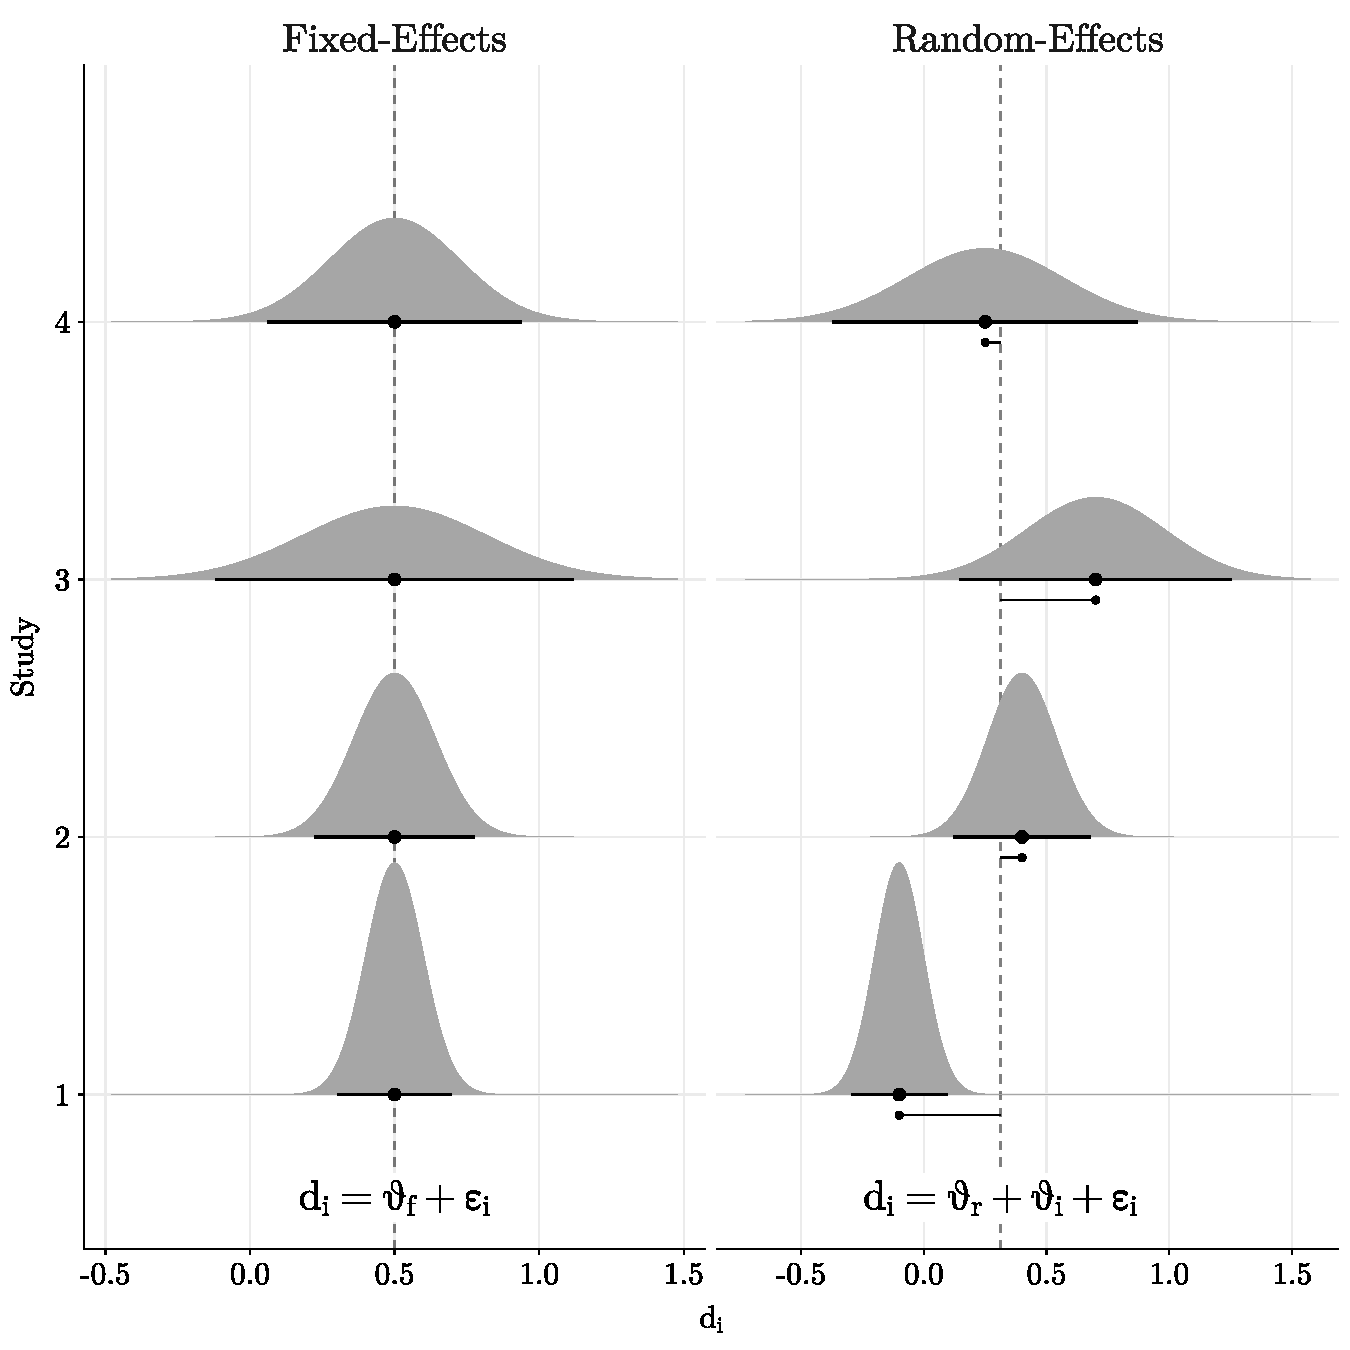
\includegraphics[width=0.8\linewidth]{paper_files/figure-latex/img-fixed-vs-random-1} 

}

\caption{The difference between the assumptions of the \emph{fixed} and \emph{random-effects model}. Each distribution depicts the sampling distribution of \(k = 4\) hypothetical studies (\(i = 1\), \(2\), \ldots, \(4\)) with a certain observed effect size \(d_{i}\), sampling variability \(\sigma_{i}^{2}\) and the 95\% confidence interval (black segment). The \emph{fixed-effects} plot on the left suggests that each observed effect size has the same underlying true effect \(\theta_{f}\) (each distribution has the same mean) with a different degree of precision (e.g., Study 1 is more precise than Study 3). In practice, each study has a different observed effect size where studies with high precision (i.e., narrow sampling distributions) will be remarkably close to the real effect (\(\theta_{f}\)). The \emph{random-effects model} on the right suggests that beyond the error term (\(\epsilon_{i}\)), each real effect size is composed of a fixed part (now \(\theta_{r}\)) and a random part (\(\theta_{i}\), black segments below the sampling distributions). The random part is determined by \(\tau^{2}\), which represents the variability of the effect size distribution at the population level. When \(\tau^{2}\) is zero, the random-effects reduces to a fixed-effects model.}\label{fig:img-fixed-vs-random}
\end{figure}

\normalsize

\hypertarget{multilevel-and-multivariate-models}{%
\subsubsection{Multilevel and multivariate models}\label{multilevel-and-multivariate-models}}

The most straightforward situation for a meta-analysis is when each included study contributes with a single effect size. However, it is common to have multiple effect sizes belonging to the same study creating a situation of dependency between statistical units. There are numerous sources of dependency for a meta-analysis (Cheung, 2014; 2015, pp. 121--122). The first type of dependency (\emph{multilevel}) consists of multiple effect sizes from independent participants. Despite being collected with different participants, effect sizes from the same study could be correlated. We obtain a multilevel data structure with independent effect sizes in the same study. There are multiple ways to model this data structure (see Cheung, 2014 for an overview). Still, the most common way is to use a \emph{multilevel meta-analysis model,} considering the heterogeneity between and within studies. The standard \emph{random-effects} (but also the \emph{fixed-effects model}) model is also called a \emph{two-level} model because it combines data after aggregating the participants-level (\emph{first-level}) data. The \emph{three-level} model is commonly used to manage the multilevel data structure (Cheung, 2014, 2019). Compared to the \emph{two-level} model, the \emph{three-level} model estimates two heterogeneity parameters (\(\tau^{2}\) and \(\omega^{2}\)), one for the heterogeneity between studies and the other for the heterogeneity within studies.

A second type of dependency (\emph{multivariate}) consists of multiple effect sizes collected from the same pool of participants. For example, when using two cognitive tasks on the same pool of participants. This is commonly known as \emph{multivariate meta-analysis} because the effect sizes sampling errors are correlated given that participants are assessed multiple times. A \emph{multivariate meta-analysis model} could be used to
consider the correlation between sampling errors.

A third type of dependency arises when true effect sizes are correlated at the population level (Cheung, 2015, pp. 121--122). For example, two different memory tasks could be correlated because the latent psychological constructs are intrinsically correlated. This correlation is present even when other groups of participants perform the two memory tasks (i.e., no \emph{multivariate} dependency) or are administered by different researchers (i.e., no \emph{multilevel} dependency). This type of dependency could be managed by estimating the correlation between outcomes using a \emph{multivariate random-effects model} (Cheung, 2015, pp. 127--130). Figures \ref{fig:img-multilevel} and \ref{fig:img-multivariate} depict the conceptual idea of \emph{multilevel} and \emph{multivariate} models.

\scriptsize

\begin{figure}[H]

{\centering 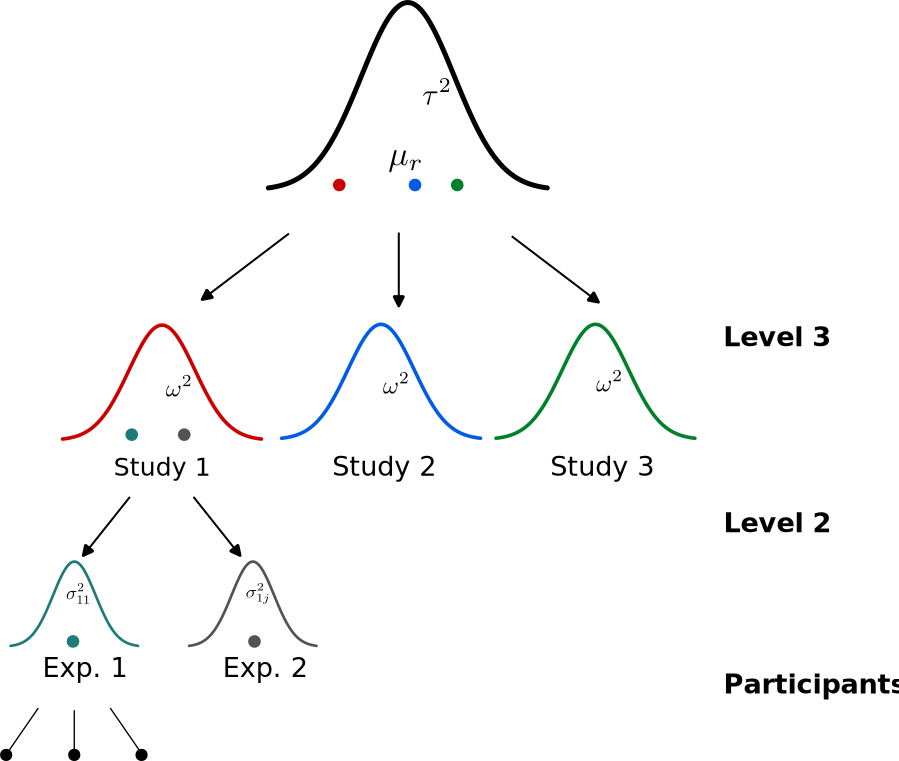
\includegraphics[width=0.8\linewidth]{img/multilevel} 

}

\caption{Graphical representation of a \emph{multilevel} (three-level) model. On the top, the effect sizes are distributed at the population level. Then, each study is defined as the overall effect and the random effects determined by \(\tau^{2}\), \(\theta_{r} + \theta_{i}\). Finally, each experiment (effect size) within a study is composed of the study-specific effect \(\theta_{r} + \theta_{i}\) and the experiment-specific random-effects \(\theta_{r} + \theta_{i} + \theta_{\text{ij}}\) determined by \(\omega^{2}\).}\label{fig:img-multilevel}
\end{figure}

\normalsize

\scriptsize

\begin{figure}[H]

{\centering 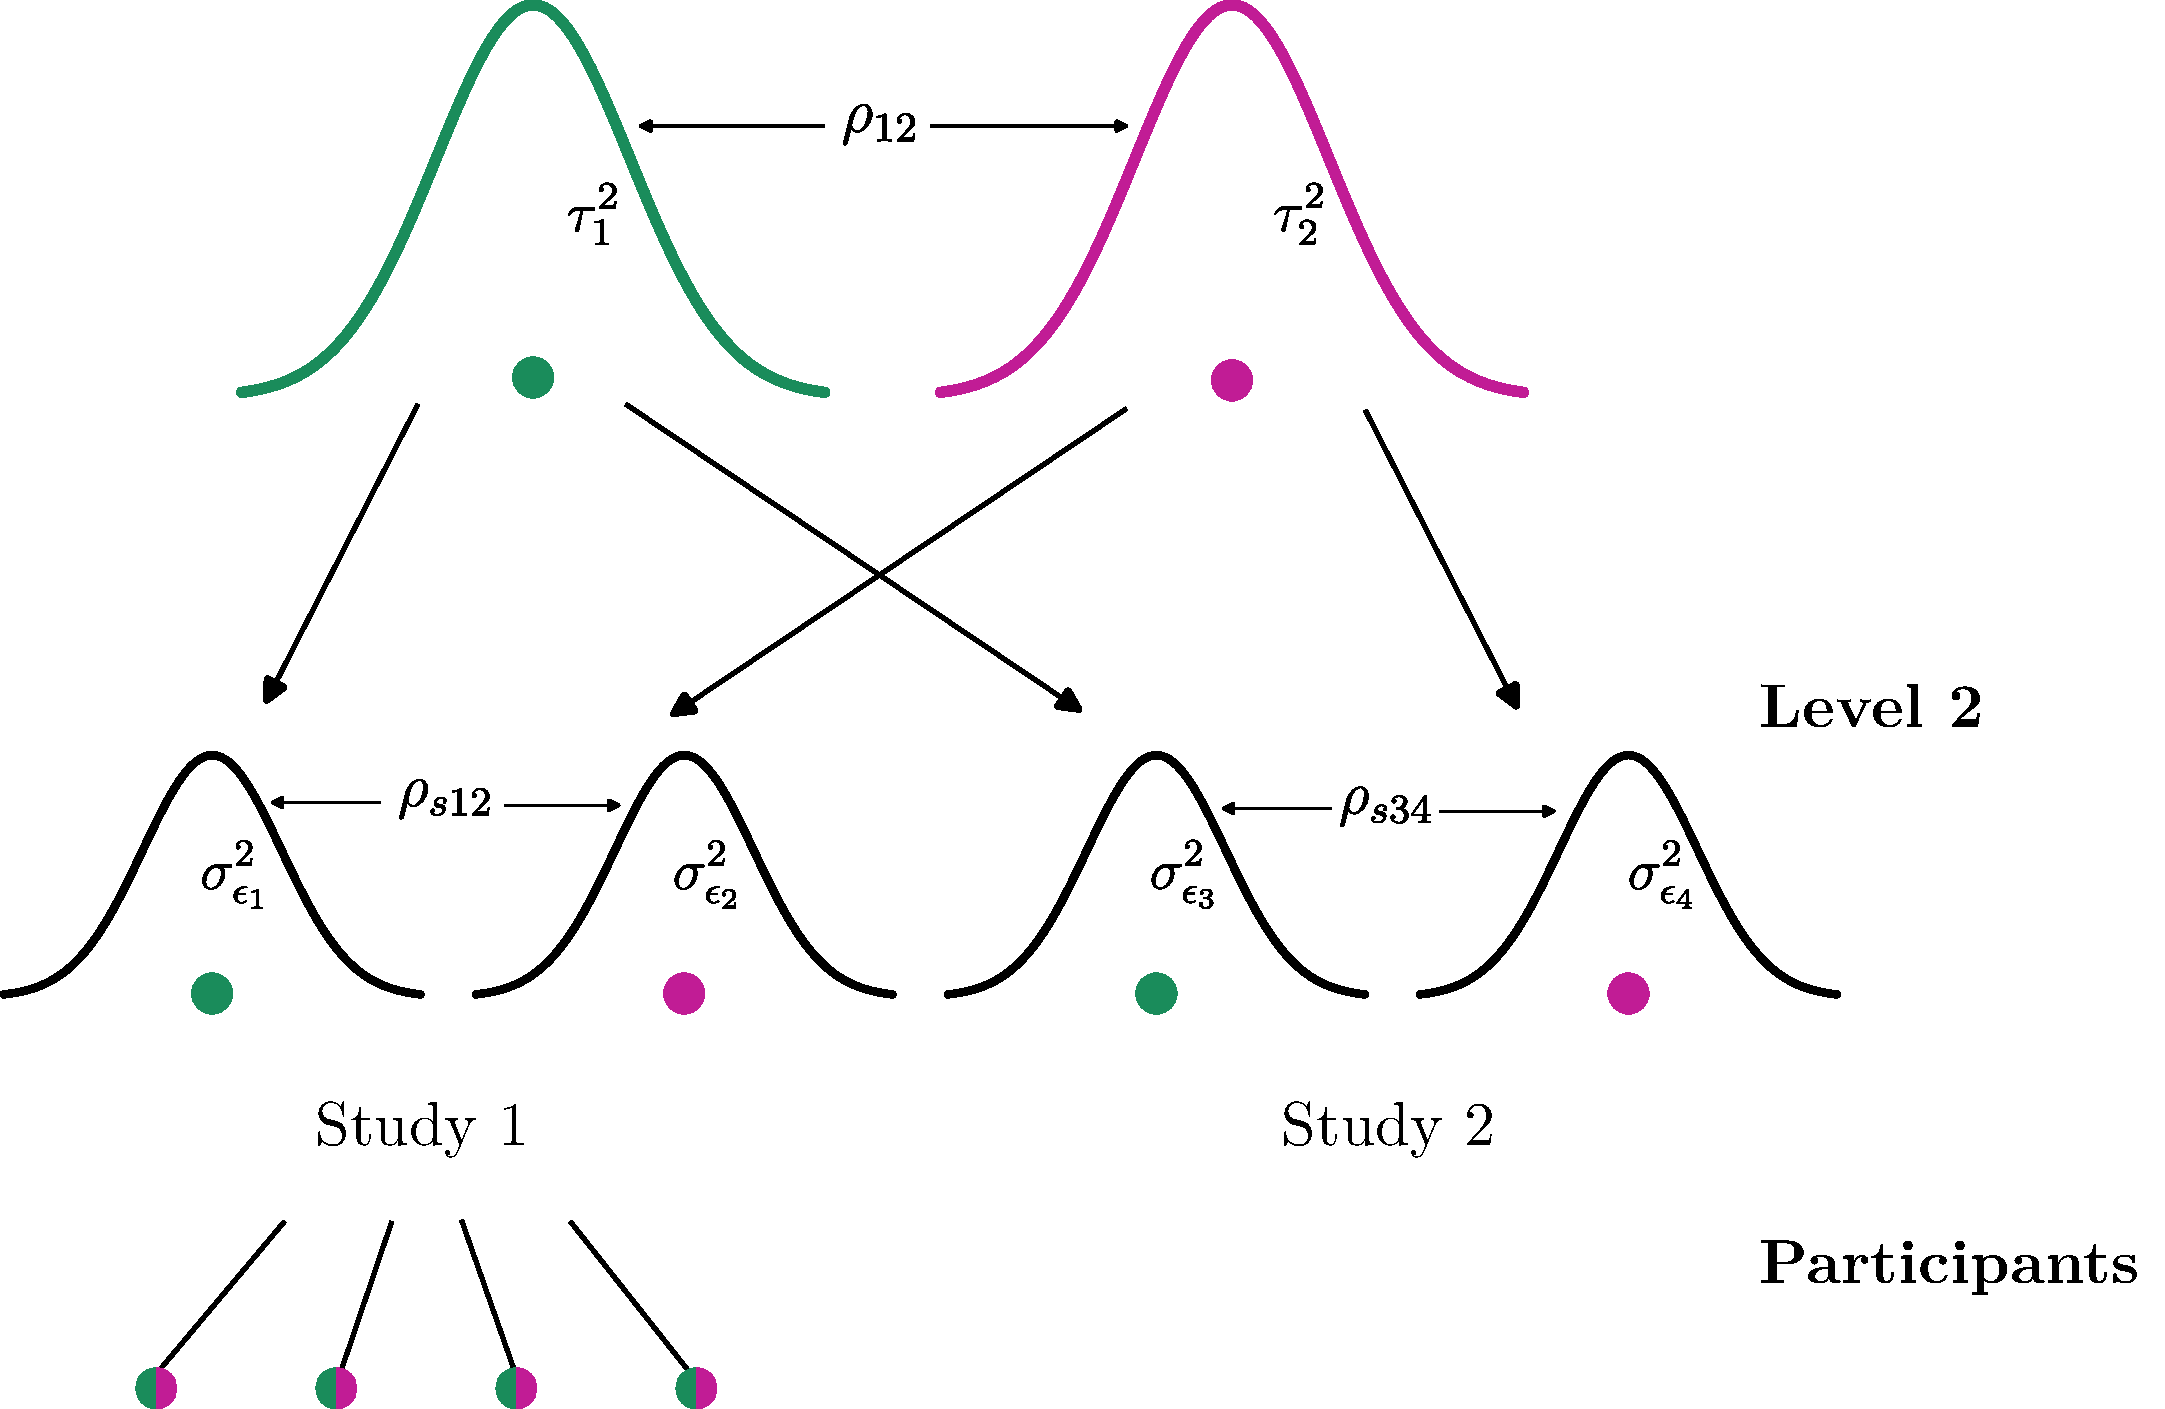
\includegraphics[width=0.8\linewidth]{img/multivariate.pdf } 

}

\caption{Graphical representation of a \emph{multivariate} model. In this example, we have two outcomes (magenta and green) with an average effect, heterogeneity parameters, and a certain true correlation value (\(\rho\), third type of dependency). Each study at level-2 (as in the standard random-effects model) has two effect sizes with corresponding sampling variances. The two effect sizes are correlated (\(\rho_{s}\), with \(s\) for sampling errors) because each effect is collected on the same participants.}\label{fig:img-multivariate}
\end{figure}

\normalsize

\hypertarget{simulation}{%
\section{Simulation}\label{simulation}}

\hypertarget{monte-carlo-simulations}{%
\subsection{Monte Carlo simulations}\label{monte-carlo-simulations}}

The Monte Carlo methods are controlled experiments (Gentle, 2009). Given a set of fixed parameters, probability distributions, and the possibility of generating random numbers, it is possible to simulate the behavior of an empirical system. Monte Carlo simulations are used for statistical and mathematical problems that cannot be solved analytically.

A straightforward example regards estimating the sampling variability of the mean difference. When calculating the mean difference between two samples, we estimate the true mean difference at the population level with a certain degree of error (i.e., the standard error of the mean difference). The central limit theorem states that the difference between the means of two random samples (\(\overline{X}\) and \(\overline{Y}\)) is approximately normally distributed with mean \(\mu_{x} - \mu_{y}\) and standard error \(\sqrt{\frac{\sigma^2_x}{{n_x}} + \frac{\sigma^2_y}{{n_y}}}\). The same results can be obtained using Monte Carlo simulations using the following procedure:

\begin{enumerate}
\def\labelenumi{\arabic{enumi}.}
\tightlist
\item
  Generating two random samples from two normal distributions with a fixed mean difference
\item
  Calculating the mean difference
\item
  Repeating the same process, many times
\item
  Calculate the standard deviation of the simulated values
\end{enumerate}

Using the method, we are estimating via simulation the standard deviation of the sampling distribution of the mean difference (i.e., the standard error of the mean difference). Increasing the number of simulations will produce more stable results.

\scriptsize

\begin{Shaded}
\begin{Highlighting}[]
\FunctionTok{set.seed}\NormalTok{(}\DecValTok{123}\NormalTok{) }\CommentTok{\# seed for simulation to ensure the reproducibility of results}
\NormalTok{theta }\OtherTok{\textless{}{-}} \FloatTok{0.5} \CommentTok{\# real mean difference in the populations}
\NormalTok{sigma }\OtherTok{\textless{}{-}} \DecValTok{1} \CommentTok{\# real standard deviations in the population}
\NormalTok{n }\OtherTok{\textless{}{-}} \DecValTok{30} \CommentTok{\# sample size for both groups}
\NormalTok{nsims }\OtherTok{\textless{}{-}} \FloatTok{1e5} \CommentTok{\# number of simulations = 100000}

\CommentTok{\# simulates the sampling distribution of the mean difference}
\NormalTok{d\_mc }\OtherTok{\textless{}{-}} \FunctionTok{replicate}\NormalTok{(nsims, }\AttributeTok{expr =}\NormalTok{ \{}
\NormalTok{  g1 }\OtherTok{\textless{}{-}} \FunctionTok{rnorm}\NormalTok{(}\AttributeTok{n =}\NormalTok{ n, }\AttributeTok{mean =}\NormalTok{ theta, }\AttributeTok{sd =}\NormalTok{ sigma)}
\NormalTok{  g2 }\OtherTok{\textless{}{-}} \FunctionTok{rnorm}\NormalTok{(}\AttributeTok{n =}\NormalTok{ n, }\AttributeTok{mean =} \DecValTok{0}\NormalTok{, }\AttributeTok{sd =}\NormalTok{ sigma)}
  \FunctionTok{mean}\NormalTok{(g1) }\SpecialCharTok{{-}} \FunctionTok{mean}\NormalTok{(g2) }\CommentTok{\# calculates the sample mean difference and returns the value}
\NormalTok{\})}

\CommentTok{\# analytical standard error of the mean difference}
\NormalTok{se\_an }\OtherTok{\textless{}{-}} \FunctionTok{sqrt}\NormalTok{(sigma}\SpecialCharTok{\^{}}\DecValTok{2}\SpecialCharTok{/}\NormalTok{n }\SpecialCharTok{+}\NormalTok{ sigma}\SpecialCharTok{\^{}}\DecValTok{2}\SpecialCharTok{/}\NormalTok{n)}

\CommentTok{\# monte{-}carlo standard error of the mean difference}
\NormalTok{se\_mc }\OtherTok{\textless{}{-}} \FunctionTok{sd}\NormalTok{(d\_mc)}
\end{Highlighting}
\end{Shaded}

\normalsize

The standard error estimated solving analytically is 0.26 and using the Monte Carlo simulation we arrive at the same result (i.e., 0.26).

\hypertarget{simulation-setup}{%
\subsection{Simulation setup}\label{simulation-setup}}

We load relevant packages and set the \texttt{seed} for reproducibility to prepare the R environment for the simulations.

\scriptsize

\begin{Shaded}
\begin{Highlighting}[]
\FunctionTok{library}\NormalTok{(dplyr) }\CommentTok{\# for data manipulation}
\FunctionTok{library}\NormalTok{(tidyr) }\CommentTok{\# for data manipulation}
\FunctionTok{library}\NormalTok{(metafor) }\CommentTok{\# for meta{-}analysis models fitting}
\NormalTok{seed }\OtherTok{\textless{}{-}} \DecValTok{2023} \CommentTok{\# general seed for all simulations}
\end{Highlighting}
\end{Shaded}

\normalsize

Before diving into the specific simulations, in this section, we define the common aspects of all simulations in the following sections. The current paper focuses on the \emph{two-level}, \emph{fixed,} and \emph{random-effects model}s. All the examples refer to primary studies that assess the efficacy of a treatment by comparing a control and an experimental group. Equation \eqref{eq:datagen} formalizes the assumption about generating participants' data within a single study. The two groups (\emph{experimental} \(y_{T}\) and \emph{control} \(y_{C}\)) are generated from normal distributions with \(\mu = 0\) for the control group and \(\mu = \theta\) (where \(\theta\) is the effect size) for the experimental group. Both groups are assumed to be sampled from populations with homogeneous variances \(\sigma^{2} = 1\).

\begin{align}
\begin{gathered}
y_{Ti} \sim \mathcal{N}(\theta, 1) \\
y_{Ci} \sim \mathcal{N}(0, 1)
\label{eq:datagen}
\end{gathered}
\end{align}

The true Standardized Mean Difference can be estimated using Cohen's \(d\) as reported in Equation \eqref{eq:effsize}. The difference between the two means is divided by the pooled standard deviation of the two groups. It is common to apply a small-sample correction version of this effect size called Hedges' \(g\) (Hedges, 1981)

\begin{align}
\begin{gathered}
d = \frac{\bar y_T - \bar y_C}{S_p} \\
S_p = \sqrt{\frac{S^2_{y_T}(n_{y_T} - 1) + S^2_{y_C}(n_{C} - 1)}{n_{T} + n_{C} - 2}} \\
\sigma^2_d = \frac{n_{T} + n_{C}}{n_{T}n_{C}} + \frac{d^2}{2(n_{T} + n_{C} - 2)}
\label{eq:effsize}
\end{gathered}
\end{align}

We can use the following algorithm implemented in the \texttt{sim\_study()} function to simulate a single study. Before using the \texttt{sim\_study()}
function, we can create a data frame for the simulation using the \texttt{make\_data()} function\footnote{This function is a simple wrapper of \texttt{data.frame()} that given the number of studies and other variables create the data structure for the simulation.}. Table \ref{tab:sim-data-example-tab} depicts an example of the \texttt{make\_data()} output.

\begin{enumerate}
\def\labelenumi{\arabic{enumi}.}
\tightlist
\item
  Choose a \(\theta\), \(n_{T}\), and \(n_{C}\) value.
\item
  Simulate \(n_{T}\) observations from a Gaussian distribution with \(\mu = \theta\) and \(\sigma^{2} = 1\) and \(n_{T}\) observations from a Gaussian distribution with \(\mu = 0\) and \(\sigma^{2} = 1\). This way, the expected difference between groups will be \(d\) and the variance is fixed at 1.
\item
  Calculate the pooled standard deviation \(S_{p}\) that is an estimation of the population standard deviation (\(\sigma\)) to standardize the mean difference.
\item
  Calculate the observed effect size \(d\) and the sampling variance \(\sigma_{d}^{2}\).
\end{enumerate}

\scriptsize

\begin{Shaded}
\begin{Highlighting}[]

\NormalTok{make\_data }\OtherTok{\textless{}{-}} \ControlFlowTok{function}\NormalTok{(k, }\AttributeTok{nt =} \ConstantTok{NULL}\NormalTok{, }\AttributeTok{nc =} \ConstantTok{NULL}\NormalTok{, ...)\{}
\NormalTok{  params }\OtherTok{\textless{}{-}} \FunctionTok{c}\NormalTok{(}\FunctionTok{as.list}\NormalTok{(}\FunctionTok{environment}\NormalTok{()), }\FunctionTok{list}\NormalTok{(...))}
\NormalTok{  cols }\OtherTok{\textless{}{-}}\NormalTok{ params[}\SpecialCharTok{!}\FunctionTok{sapply}\NormalTok{(params, is.null) }\SpecialCharTok{\&} \FunctionTok{names}\NormalTok{(params) }\SpecialCharTok{!=} \StringTok{"k"}\NormalTok{]}
\NormalTok{  dat }\OtherTok{\textless{}{-}} \FunctionTok{data.frame}\NormalTok{(}
    \AttributeTok{id =} \DecValTok{1}\SpecialCharTok{:}\NormalTok{params}\SpecialCharTok{$}\NormalTok{k}
\NormalTok{  )}
  \ControlFlowTok{if}\NormalTok{(}\FunctionTok{length}\NormalTok{(cols) }\SpecialCharTok{!=} \DecValTok{0}\NormalTok{)\{}
\NormalTok{    dat }\OtherTok{\textless{}{-}} \FunctionTok{cbind}\NormalTok{(dat, cols)}
\NormalTok{  \}}
  \FunctionTok{return}\NormalTok{(dat)}
\NormalTok{\}}
\end{Highlighting}
\end{Shaded}

\normalsize

\scriptsize

\begin{Shaded}
\begin{Highlighting}[]

\NormalTok{sim\_study }\OtherTok{\textless{}{-}} \ControlFlowTok{function}\NormalTok{(theta, nt, }\AttributeTok{nc =} \ConstantTok{NULL}\NormalTok{, }\AttributeTok{hedges =} \ConstantTok{TRUE}\NormalTok{, }\AttributeTok{aggregate =} \ConstantTok{TRUE}\NormalTok{)\{}
  \ControlFlowTok{if}\NormalTok{(}\FunctionTok{is.null}\NormalTok{(nc)) nc }\OtherTok{\textless{}{-}}\NormalTok{ nt}
  \CommentTok{\# generate from normal distribution}
\NormalTok{  yc }\OtherTok{\textless{}{-}} \FunctionTok{rnorm}\NormalTok{(nc, }\DecValTok{0}\NormalTok{, }\DecValTok{1}\NormalTok{)}
\NormalTok{  yt }\OtherTok{\textless{}{-}} \FunctionTok{rnorm}\NormalTok{(nt, theta, }\DecValTok{1}\NormalTok{)}
  \CommentTok{\# pooled variance}
\NormalTok{  sp }\OtherTok{\textless{}{-}} \FunctionTok{sqrt}\NormalTok{((}\FunctionTok{var}\NormalTok{(yc)}\SpecialCharTok{*}\NormalTok{(nc }\SpecialCharTok{{-}} \DecValTok{1}\NormalTok{) }\SpecialCharTok{+} \FunctionTok{var}\NormalTok{(yt)}\SpecialCharTok{*}\NormalTok{(nt }\SpecialCharTok{{-}} \DecValTok{1}\NormalTok{)) }\SpecialCharTok{/}\NormalTok{ (nc }\SpecialCharTok{+}\NormalTok{ nt }\SpecialCharTok{{-}} \DecValTok{2}\NormalTok{))}
  \CommentTok{\# effect size}
\NormalTok{  yi }\OtherTok{\textless{}{-}}\NormalTok{ (}\FunctionTok{mean}\NormalTok{(yt) }\SpecialCharTok{{-}} \FunctionTok{mean}\NormalTok{(yc)) }\SpecialCharTok{/}\NormalTok{ sp}
  
  \CommentTok{\# transform to hedges\textquotesingle{} g}
  \ControlFlowTok{if}\NormalTok{(hedges)\{}
\NormalTok{    yi }\OtherTok{\textless{}{-}}\NormalTok{ yi }\SpecialCharTok{*}\NormalTok{ metafor}\SpecialCharTok{:::}\FunctionTok{.cmicalc}\NormalTok{(nc }\SpecialCharTok{+}\NormalTok{ nt }\SpecialCharTok{{-}} \DecValTok{2}\NormalTok{)}
\NormalTok{  \}}
  
  \CommentTok{\# sampling variance}
\NormalTok{  vi }\OtherTok{\textless{}{-}}\NormalTok{ (nc }\SpecialCharTok{+}\NormalTok{ nt)}\SpecialCharTok{/}\NormalTok{(nc }\SpecialCharTok{*}\NormalTok{ nt) }\SpecialCharTok{+}\NormalTok{ yi}\SpecialCharTok{\^{}}\DecValTok{2}\SpecialCharTok{/}\NormalTok{(}\DecValTok{2} \SpecialCharTok{*}\NormalTok{ (nc }\SpecialCharTok{+}\NormalTok{ nt }\SpecialCharTok{{-}} \DecValTok{2}\NormalTok{))}
  
  \ControlFlowTok{if}\NormalTok{(}\SpecialCharTok{!}\NormalTok{aggregate)\{}
    \CommentTok{\# return raw data}
    \FunctionTok{data.frame}\NormalTok{(}\AttributeTok{id =} \DecValTok{1}\SpecialCharTok{:}\NormalTok{(nc }\SpecialCharTok{+}\NormalTok{ nt),}
               \AttributeTok{group =} \FunctionTok{rep}\NormalTok{(}\FunctionTok{c}\NormalTok{(}\StringTok{"c"}\NormalTok{, }\StringTok{"t"}\NormalTok{), }\FunctionTok{c}\NormalTok{(nc, nt)),}
               \AttributeTok{y =} \FunctionTok{c}\NormalTok{(yc, yt))}
\NormalTok{  \}}\ControlFlowTok{else}\NormalTok{\{}
    \CommentTok{\# compute effect size}
    \FunctionTok{data.frame}\NormalTok{(yi, vi)}
\NormalTok{  \}}
\NormalTok{\}}

\NormalTok{sim\_studies }\OtherTok{\textless{}{-}} \ControlFlowTok{function}\NormalTok{(..., }\AttributeTok{data =} \ConstantTok{NULL}\NormalTok{)\{}
  \CommentTok{\# ... (dots) are the arguments passed to mapply, with the order required by sim\_study}
\NormalTok{  res }\OtherTok{\textless{}{-}} \FunctionTok{mapply}\NormalTok{(sim\_study, ..., }\AttributeTok{SIMPLIFY =} \ConstantTok{FALSE}\NormalTok{)}
  \CommentTok{\# everything to a dataframe}
\NormalTok{  res }\OtherTok{\textless{}{-}}\NormalTok{ dplyr}\SpecialCharTok{::}\FunctionTok{bind\_rows}\NormalTok{(res)}
  
  \ControlFlowTok{if}\NormalTok{(}\SpecialCharTok{!}\FunctionTok{is.null}\NormalTok{(data))\{}
    \CommentTok{\# attach to the original dataset}
    \FunctionTok{cbind}\NormalTok{(data, res)}
\NormalTok{  \}}\ControlFlowTok{else}\NormalTok{\{}
\NormalTok{    res}
\NormalTok{  \}}
\NormalTok{\}}
\end{Highlighting}
\end{Shaded}

\normalsize

The \texttt{theta} is the true effect size, \texttt{nc} and \texttt{nt} are the sample size for the control and experimental group, \texttt{aggregate} controls if returning the effect size and the corresponding variance or the participant-level data, and \texttt{hedges} specify whether applying the correction. We can generate a single study with the desired parameters with this function. A suggestion for each simulation step is to generate a large \(n\) to reduce the sampling error and check the recovery of simulated parameters. This is a general strategy that can be applied to every simulation. The \texttt{sim\_studies()} function will iterate through variables in the \texttt{...} argument creating the meta-analysis data frame. The \texttt{mapply()} function is clearly explained in the supplementary materials.

The following code simulates a single study with \(n = 10000\) and check the estimated mean and standard deviation.

\scriptsize

\begin{Shaded}
\begin{Highlighting}[]
\FunctionTok{set.seed}\NormalTok{(seed)}
\FunctionTok{sim\_study}\NormalTok{(}\AttributeTok{theta =} \FloatTok{0.3}\NormalTok{, }\AttributeTok{nc =} \DecValTok{10000}\NormalTok{, }\AttributeTok{nt =} \DecValTok{10000}\NormalTok{, }\AttributeTok{aggregate =} \ConstantTok{FALSE}\NormalTok{)}
\end{Highlighting}
\end{Shaded}

\normalsize

\scriptsize

\normalsize

The control group has a mean of -0.008 (SD = 0.996) and the experimental group has a mean of 0.306 (SD = 1.013) which are remarkably close to the simulated values.

Using the \texttt{sim\_study()} function multiple times (with the appropriate adjustments) we can generate a series of studies simulating a data set for a meta-analysis (using the \texttt{sim\_studies()} function). After each example, we will compute the appropriate model (e.g., \emph{fixed} or \emph{random-effects}) using the \texttt{metafor} package (Viechtbauer, 2010) to check the recovery of simulated parameters. Table \ref{tab:notation-tab} summarizes the simulation parameters notation in equations and code.

\scriptsize

\begin{Shaded}
\begin{Highlighting}[]
\NormalTok{k }\OtherTok{\textless{}{-}} \DecValTok{30} \CommentTok{\# number of studies}
\NormalTok{n }\OtherTok{\textless{}{-}} \DecValTok{20} \CommentTok{\# number of participants per group, per study}
\NormalTok{theta }\OtherTok{\textless{}{-}} \FloatTok{0.3} \CommentTok{\# real effect size}
\NormalTok{sim }\OtherTok{\textless{}{-}} \FunctionTok{make\_data}\NormalTok{(}\AttributeTok{k =}\NormalTok{ k, }\AttributeTok{nt =}\NormalTok{ n, }\AttributeTok{nc =}\NormalTok{ n, }\AttributeTok{theta =}\NormalTok{ theta)}
\end{Highlighting}
\end{Shaded}

\normalsize

\scriptsize

\begin{table}[H]

\begin{center}
\begin{threeparttable}

\caption{\label{tab:sim-data-example-tab}Example of data generated with the \texttt{make\_data()} function. The \texttt{id} column is the identifier for each study.}

\small{

\begin{tabular}{llll}
\toprule
id & \multicolumn{1}{c}{nt} & \multicolumn{1}{c}{nc} & \multicolumn{1}{c}{theta}\\
\midrule
1 & 20 & 20 & 0.3\\
2 & 20 & 20 & 0.3\\
... & ... & ... & ...\\
29 & 20 & 20 & 0.3\\
30 & 20 & 20 & 0.3\\
\bottomrule
\end{tabular}

}

\end{threeparttable}
\end{center}

\end{table}

\normalsize

\scriptsize

\begin{table}[H]

\begin{center}
\begin{threeparttable}

\caption{\label{tab:notation-tab}Variables in the data-generating model and associated R code.}

\begin{tabular}{lll}
\toprule
Equation & \multicolumn{1}{c}{Code} & \multicolumn{1}{c}{Description}\\
\midrule
$\theta_f$ & \texttt{theta\_f} & Fixed-effects model real effect size\\
$\theta_r$ & \texttt{theta\_r} & Random-effects model real effect size\\
$\tau^2$ & \texttt{tau2} & Effect size heterogeneity\\
$\tau^2_r$ & \texttt{tau2r} & Residual effect size heterogeneity\\
$\bar y_{T, C}$ & \texttt{} & Mean of the experimental/control group\\
$s^2_{T, C}$ & \texttt{} & Standard deviation of the experimental/control group\\
$n_{T, C}$ & \texttt{nt, nc} & Sample size of the experimental/control group\\
$d_i$ & \texttt{yi} & Observed effect size\\
$\sigma^2_i$ & \texttt{vi} & Observed sampling variance\\
$\theta_i$ & \texttt{theta\_i} & Random effect for the study i\\
$\beta_0$ & \texttt{b0} & Meta-regression intercept\\
$\beta_1$ & \texttt{b1} & Meta-regression slope\\
$k$ & \texttt{k} & Number of studies\\
$\epsilon_i$ & \texttt{} & Sampling error for the study i\\
\bottomrule
\addlinespace
\end{tabular}

\begin{tablenotes}[para]
\normalsize{\textit{Note.} The \texttt{yi} and \texttt{vi} notation for the observed effect size ($d_i$) and sampling variance ($\sigma^2_i$) has been used to be consistent with the \texttt{metafor} notation.}
\end{tablenotes}

\end{threeparttable}
\end{center}

\end{table}

\normalsize

\hypertarget{fixed-effects-model}{%
\subsection{Fixed-effects model}\label{fixed-effects-model}}

The most basic model to simulate is the \emph{fixed-effects model} (FE). As reported in the previous sections, the \emph{fixed-effects model} assumes the presence of a single true effect (\(\theta_{f}\)) and the observed variability is because each effect size is an imprecise estimation of the true effect. In other words, the only source of variability is the sampling variability that depends on the variance of the primary studies
(i.e., the sample size). Equation \eqref{eq:fixed-effect-model} depicts the \emph{fixed-effect} equation.

\begin{align}
\begin{gathered}
d_i = \theta_f + \epsilon_i \\
\epsilon_i \sim \mathcal{N}(0,\sigma^2_i)
\label{eq:fixed-effect-model}
\end{gathered}
\end{align}

Each observed effect size (\(d_{i}\)) is composed of the real effect size \(\theta_{f}\) plus an error term (\(\epsilon_{i}\)) that is sampled from a normal distribution with \(\mu = 0\) and \(\sigma^{2} = \sigma_{i}^{2}\) (i.e., the known sampling variance of the study \(i\)). As demonstrated in
Equation \eqref{eq:effsize}, the increase in sample size will decrease the sampling variability. An exact study will essentially have \(\theta_{f}\) as the observed effect size. Since we are sampling participants' level data, the error component is already included in the \texttt{sim\_study()} function. To simulate this model in R we can just call the \texttt{sim\_study()} multiple times according to the number of desired studies (\(k\)). In addition, we simulate that each primary study will have a sample size of \(n = 20\) for both groups. We will discuss later the appropriateness of this assumption.

\scriptsize

\begin{Shaded}
\begin{Highlighting}[]
\FunctionTok{set.seed}\NormalTok{(seed)}
\NormalTok{k }\OtherTok{\textless{}{-}} \DecValTok{30} \CommentTok{\# number of studies}
\NormalTok{n }\OtherTok{\textless{}{-}} \DecValTok{20} \CommentTok{\# number of participants per group, per study}
\NormalTok{theta\_f }\OtherTok{\textless{}{-}} \FloatTok{0.3} \CommentTok{\# real effect size}

\NormalTok{sim }\OtherTok{\textless{}{-}} \FunctionTok{make\_data}\NormalTok{(}\AttributeTok{k =}\NormalTok{ k, }\AttributeTok{nt =}\NormalTok{ n, }\AttributeTok{nc =}\NormalTok{ n, }\AttributeTok{theta\_f =}\NormalTok{ theta\_f)}
\NormalTok{sim }\OtherTok{\textless{}{-}} \FunctionTok{sim\_studies}\NormalTok{(sim}\SpecialCharTok{$}\NormalTok{theta\_f, sim}\SpecialCharTok{$}\NormalTok{nc, sim}\SpecialCharTok{$}\NormalTok{nt, }\AttributeTok{data =}\NormalTok{ sim) }\CommentTok{\# simulated data}
\NormalTok{res }\OtherTok{\textless{}{-}} \FunctionTok{rma}\NormalTok{(}\AttributeTok{yi =}\NormalTok{ yi, }\AttributeTok{vi =}\NormalTok{ vi, }\AttributeTok{method =} \StringTok{"FE"}\NormalTok{, }\AttributeTok{data =}\NormalTok{ sim)}
\end{Highlighting}
\end{Shaded}

\normalsize

We are using the \(\theta_{f}\) parameter to generate random data using the \texttt{sim\_study()} function that will introduce the random error component \(\epsilon_{i}\). Then we can fit the \emph{fixed-effects} meta-analysis model with the \texttt{rma} function and \texttt{method\ =\ "FE"} of the \texttt{metafor} package. The parameter we are estimating is \(\theta_{f}\) which is close to our simulation value (see Table \ref{tab:res-fixed-effect}). Increasing the number of studies (\(k\)) and/or the number of participants in each study (\(n\)) will improve estimation reducing the standard error.

\scriptsize

\begin{table}[H]

\caption{\label{tab:res-fixed-effect}Summary of the simulated fixed-effects model. The only estimated parameter is the average effect* \(\theta_{f}\) *with the standard error,
95\% confidence interval, and the Wald z-test. The z-test evaluates the null hypothesis that the real effect equals zero.}
\centering
\fontsize{9}{11}\selectfont
\begin{tabular}[t]{ccccc}
\toprule
 & $\beta$ & 95\% CI & z & p\\
\midrule
overall & 0.334 (SE = 0.059) & $[0.219, 0.449]$ & 5.701 & < 0.001\\
\bottomrule
\multicolumn{5}{l}{\textsuperscript{} $k = 30$}\\
\end{tabular}
\end{table}

\normalsize

Increasing the sample size for each study will increase the estimation precision thus the variability among studies will be reduced. This can be easily demonstrated by simulating studies with a high sample size as reported in Figure \ref{fig:fixed-effect-high-low-precision}. As the sample size increases the only source of variability (i.e., the error component \(\epsilon_{i}\)) is close to zero so each study is closer to the true simulated value.

\scriptsize

\begin{figure}[H]

{\centering 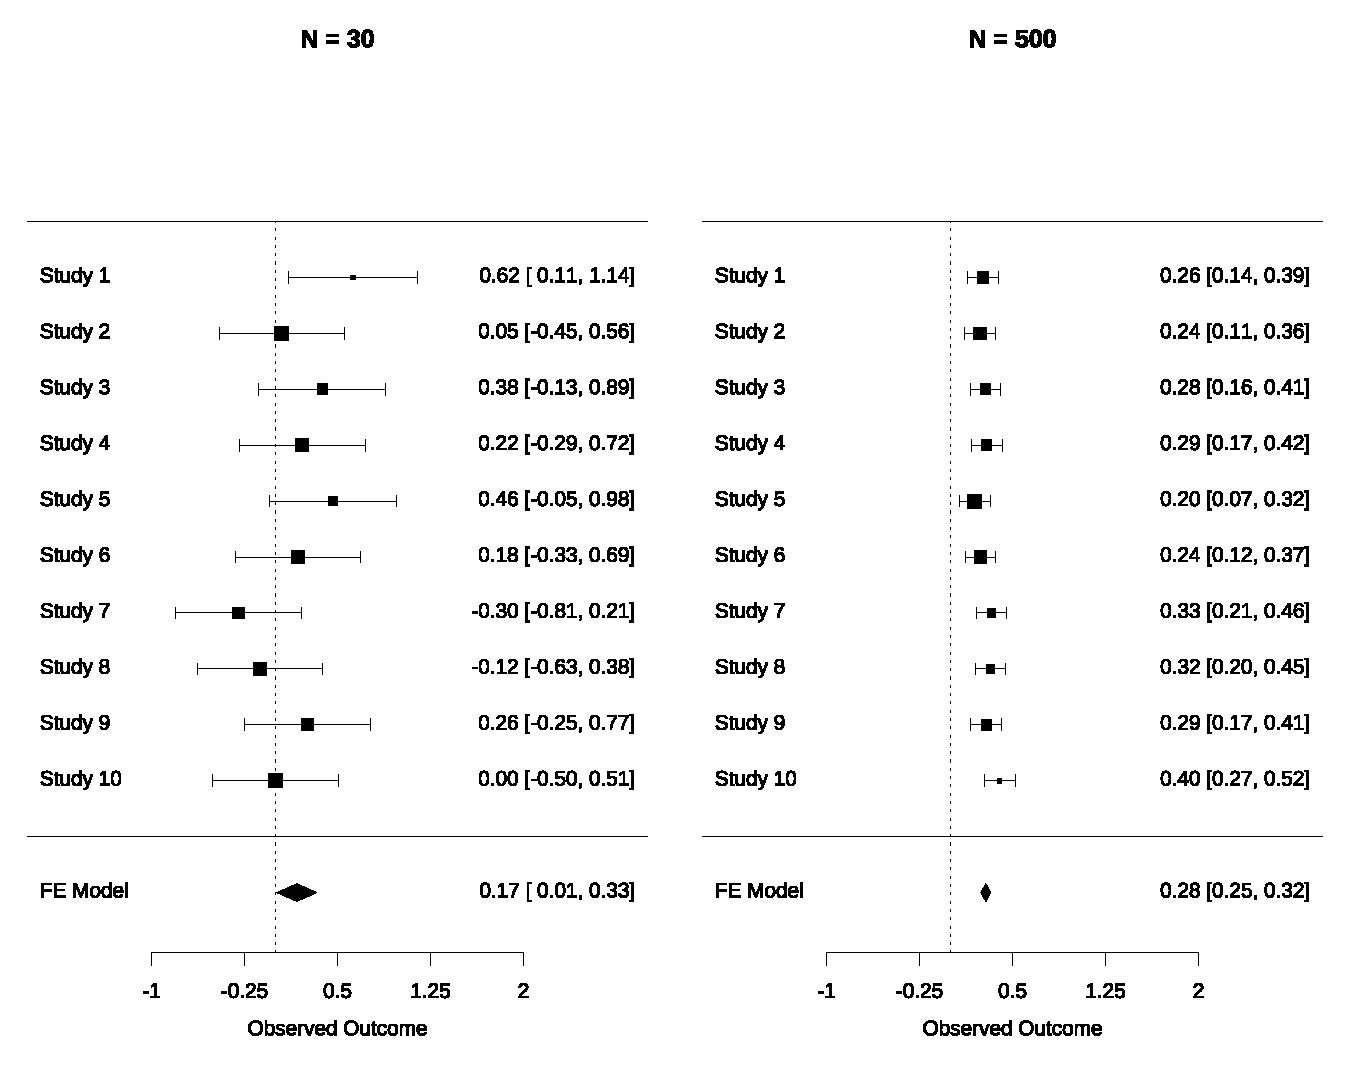
\includegraphics[width=0.8\linewidth]{paper_files/figure-latex/fixed-effect-high-low-precision-1} 

}

\caption{Forest plots of two simulated \emph{fixed-effects models}. On the left, the simulated model has \(nt,nc = 30\) for each included study while on the right the sample size for each study is \(nt,nc = 500\). Given that the data were generated under a \emph{fixed-effects model}, when the sample size is high (on the right) each study is aligned on the real effect size because the error component (\(\epsilon_{i}\)) is almost entirely reduced. The average effect size is similar (depending on the random numbers generation) between the two scenarios while the estimation precision (the width of the black diamond) is narrower on the right.}\label{fig:fixed-effect-high-low-precision}
\end{figure}

\normalsize

\hypertarget{re-model}{%
\subsection{Random-effects model}\label{re-model}}

The \emph{random-effects model} (RE) can be considered an extension of the \emph{fixed-effects model}. The \emph{fixed-effects model} assumes that the real effect is a single value. The random-effects model relaxes this assumption allowing \(\theta_{f}\) (now \(\theta_{r}\)) to vary across studies. For example, the difference between groups we are simulating could be influenced by the type of experiment or the participants' age.
Now \(\theta_{r}\) is no longer a single value but a distribution of values. Due to the effect size being a distribution, we need two parameters \(\mu\) and \(\sigma^{2}\) to describe the phenomenon. The parameter \(\theta_{r}\) average true effect is now interpreted as the average effect size across different true effect sizes and \(\sigma^{2}\) usually known as \(\tau^{2}\) is the effect size variability or heterogeneity. In practical terms, we now have two sources of variability: \(\tau^{2}\), which express the real difference among effect sizes, and \(\sigma_{i}^{2}\) which is the known sampling variance of each study as in the \emph{fixed-effects model}. We can easily extend Equation \eqref{eq:fixed-effect-model} with Equation \eqref{eq:random-effect-model}.

\begin{align}
\begin{aligned}
d_i = \theta_r + \theta_i + \epsilon_i \\
\theta_i \sim \mathcal{N}(0, \tau^2) \\
\epsilon_i \sim \mathcal{N}(0,\sigma^2_i)
\label{eq:random-effect-model}
\end{aligned}
\end{align}

Compared to the \emph{fixed-effects model} we need to generate another adjustment to the overall effect \(\theta_{r}\) from a normal distribution with mean \(\theta_{r}\) and variance \(\tau^{2}\). The real effect size for the study \(i\) will be \(\theta_{r} + \theta_{i}\) where \(\theta_{i}\) are the random-effects regulated by the \(\tau^{2}\) parameter.

\scriptsize

\begin{Shaded}
\begin{Highlighting}[]
\FunctionTok{set.seed}\NormalTok{(seed)}
\NormalTok{k }\OtherTok{\textless{}{-}} \DecValTok{30} \CommentTok{\# number of studies}
\NormalTok{n }\OtherTok{\textless{}{-}} \DecValTok{20} \CommentTok{\# number of participants per group, per study}
\NormalTok{theta\_r }\OtherTok{\textless{}{-}} \FloatTok{0.3} \CommentTok{\# real effect size}
\NormalTok{tau2 }\OtherTok{\textless{}{-}} \FloatTok{0.2} \CommentTok{\# the effect size heterogeneity}

\NormalTok{sim }\OtherTok{\textless{}{-}} \FunctionTok{make\_data}\NormalTok{(}\AttributeTok{k =}\NormalTok{ k, }\AttributeTok{nc =}\NormalTok{ n, }\AttributeTok{nt =}\NormalTok{ n, }\AttributeTok{theta\_r =}\NormalTok{ theta\_r)}

\CommentTok{\# simulate the random{-}effects adjustment}
\NormalTok{sim}\SpecialCharTok{$}\NormalTok{theta\_i }\OtherTok{\textless{}{-}} \FunctionTok{rnorm}\NormalTok{(k, }\DecValTok{0}\NormalTok{, }\FunctionTok{sqrt}\NormalTok{(tau2))}

\CommentTok{\# adding the by{-}study adjustment to the average effect}
\NormalTok{sim}\SpecialCharTok{$}\NormalTok{theta\_r\_theta\_i }\OtherTok{\textless{}{-}}\NormalTok{ sim}\SpecialCharTok{$}\NormalTok{theta\_r }\SpecialCharTok{+}\NormalTok{ sim}\SpecialCharTok{$}\NormalTok{theta\_i }

\CommentTok{\# now we are using theta\_r\_theta\_i and no longer theta\_f}
\NormalTok{sim }\OtherTok{\textless{}{-}} \FunctionTok{sim\_studies}\NormalTok{(sim}\SpecialCharTok{$}\NormalTok{theta\_r\_theta\_i, sim}\SpecialCharTok{$}\NormalTok{nc, sim}\SpecialCharTok{$}\NormalTok{nt, }\AttributeTok{data =}\NormalTok{ sim)}
\NormalTok{res }\OtherTok{\textless{}{-}} \FunctionTok{rma}\NormalTok{(}\AttributeTok{yi =}\NormalTok{ yi, }\AttributeTok{vi =}\NormalTok{ vi, }\AttributeTok{method =} \StringTok{"REML"}\NormalTok{, }\AttributeTok{data =}\NormalTok{ sim)}
\end{Highlighting}
\end{Shaded}

\normalsize

Then we can fit the \emph{random-effects} meta-analysis model with the \texttt{rma} function and \texttt{method\ =\ "REML"}. Table \ref{tab:res-random-effect} depicts the model results\footnote{The \texttt{method\ =\ "REML"} is not the only method to estimate a random-effects model. See the \texttt{rma} documentation (\url{https://wviechtb.github.io/metafor/reference/rma.uni.html\#specifying-the-model}) for an overview of other estimation methods} of the metafor package. We are now estimating two parameters: \(\theta_{r}\) and \(\tau^{2}\). As for the \emph{fixed-effects model}, increasing the number of studies and/or the number of participants in each study will improve estimation reducing the standard error.

\scriptsize

\begin{table}[H]

\caption{\label{tab:res-random-effect}Summary of the simulated random-effects model: Compared to the fixed-effects model, there are more parameters. The \(\beta\) is the average effect (\(\theta_{r}\)) with the standard error, 95\% confidence interval, and the Wald z-test. The \(\tau^{2}\) is the estimated heterogeneity and the \(I^{2}\) (explained in Section \ref{re-model}) represents the percentage of total variability due to between-study heterogeneity.}
\centering
\fontsize{9}{11}\selectfont
\begin{tabular}[t]{ccccc}
\toprule
 & $\beta$ & 95\% CI & z & p\\
\midrule
overall & 0.381 (SE = 0.107) & $[0.172, 0.590]$ & 3.578 & < 0.001\\
\bottomrule
\multicolumn{5}{l}{\textsuperscript{} $k = 30$}\\
\multicolumn{5}{l}{\textsuperscript{} $\tau^2 = 0.234$ ($SE = 0.089$)}\\
\multicolumn{5}{l}{\textsuperscript{} $I^2 = 68.842\%$}\\
\end{tabular}
\end{table}

\normalsize

An important aspect of the \emph{random-effects model} is the interplay between the heterogeneity (\(\tau^{2}\)) and the sampling variability (\(\sigma_{i}^{2}\)). As the number of studies \(k\) increases, the estimation of \(\theta_{r}\) and \(\tau^{2}\) becomes more precise. Additionally, as each study\textquotesingle s sample size decreases, each \(\theta_{i}\) will be estimated with higher precision but as long as \(\tau^{2} \neq 0\)
there will be variability among effect sizes. In other words, increasing the sample size of each study or the number of studies will not affect the value of \(\tau^{2}\) but only the estimation precision (see Borenstein et al., 2009, Chapter 16, Figure 16.6 for a clear explanation). This can be easily demonstrated using the previous simulation, increasing each study\textquotesingle s sample size. Figure \ref{fig:random-effect-high-low-precision} depicts the same meta-analysis but with different precision in estimating the study \(d_{i}\). Compared to Figure \ref{fig:fixed-effect-high-low-precision}, increasing the sample size of primary studies improves the estimation of each study without reducing the between-studies heterogeneity.

\scriptsize

\begin{figure}[H]

{\centering 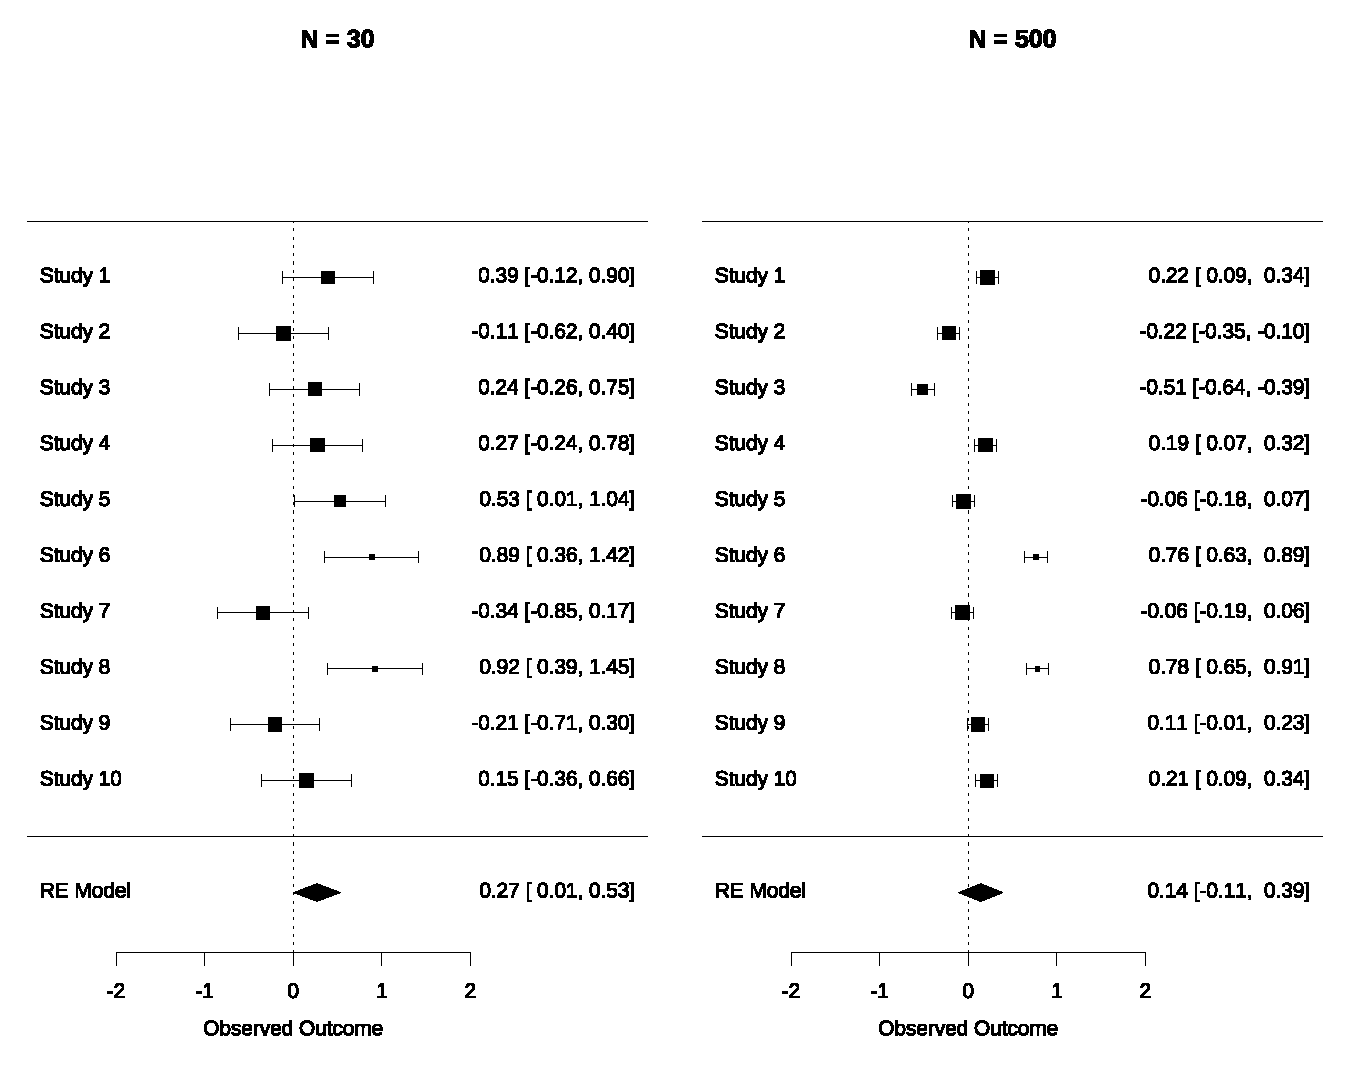
\includegraphics[width=0.8\linewidth]{paper_files/figure-latex/random-effect-high-low-precision-1} 

}

\caption{Forest plots of two simulated \emph{random-effects model}s. On the left, the simulated model has \(nt,nc = 30\) for each included study, while on the right, the sample size for each study is \(nt,nc = 500\). Compared to Figure \ref{fig:fixed-effect-high-low-precision}, data were generated under a \emph{random-effects model}. The estimated average effect is similar between the two scenarios regarding average effect and precision. However, compared to the \emph{fixed-effect} simulation, increasing the sample size of primary studies only affects the precision without reducing the true heterogeneity (i.e., \(\tau^{2} \neq 0\)).}\label{fig:random-effect-high-low-precision}
\end{figure}

\normalsize

The relationship between the sampling error and the heterogeneity can be expressed using the \(I^{2}\) statistics (e.g., Higgins \& Thompson, 2002) that is the percentage of the total variability \(\tau^{2} + \tilde{v}\) that is attributable to real heterogeneity between studies (\(\tau^{2}\)). In Equation \eqref{eq:isquared}, \(\tilde{v}\) is the ``typical'' within-study sampling variability (e.g., Higgins \& Thompson, 2002)\footnote{see also here \url{https://www.metafor-project.org/doku.php/tips:i2_multilevel_multivariate\#fn__1} for an overview of the \(I^2\) statistics also for complex models}.

\begin{align}
\begin{gathered}
I^2 = \frac{\hat{\tau}^2}{\hat{\tau}^2 + \tilde{v}}
\label{eq:isquared}
\end{gathered}
\end{align}

From Equation \eqref{eq:isquared} and Figure \ref{fig:random-effect-high-low-precision} is clear that if each included study has a considerable sample size the total variability will be reduced, mainly driven by real heterogeneity (\(\tau^2\)). This is the crucial difference between the fixed-effects and the random-effects model (see also Borenstein et al., 2009, pp. 117--122).

Given the interpretation of \(I^{2}\) it is possible to simulate a meta-analysis fixing a certain \(I^{2}\) value. The only caveat is fixing the \(\tilde{v}\). When the sample size of each study is the same, \(\tilde{v} = \sigma^2_i\). In the other case, \(\tilde{v}\) needs to be calculated from sampling variances reported in Higgins and Thompson (2002) and cannot be easily fixed a priori. However, with the assumption of homogeneous sample size across studies\footnote{The homogeneous sample size of primary studies assumption is commonly used to calculate the statistical power (see Borenstein et al., 2009, Chapter 29)}, we can solve Equation \eqref{eq:isquared} for \(\tau^{2}\) obtaining the heterogeneity value associated with a certain \(I^{2}\) as reported in Equation \eqref{eq:tau2-from-isquared}. Table \ref{tab:res-random-effect-i2} depicts the results of the random-effects model fixing the \(I^{2}\) value.

\begin{align}
\begin{gathered}
\tau^2 = - \frac{I^2\tilde{v}}{I^2 - 1}
\label{eq:tau2-from-isquared}
\end{gathered}
\end{align}

\scriptsize

\begin{Shaded}
\begin{Highlighting}[]
\FunctionTok{set.seed}\NormalTok{(seed)}
\NormalTok{k }\OtherTok{\textless{}{-}} \DecValTok{30} \CommentTok{\# number of studies}
\NormalTok{theta\_r }\OtherTok{\textless{}{-}} \FloatTok{0.3} \CommentTok{\# real effect size}
\NormalTok{n }\OtherTok{\textless{}{-}} \DecValTok{30} \CommentTok{\# sample size per group, per study}
\NormalTok{I2 }\OtherTok{\textless{}{-}} \FloatTok{0.6} \CommentTok{\# desired I2 value}

\NormalTok{v }\OtherTok{\textless{}{-}}\NormalTok{ (n }\SpecialCharTok{+}\NormalTok{ n)}\SpecialCharTok{/}\NormalTok{(n }\SpecialCharTok{*}\NormalTok{ n) }\SpecialCharTok{+}\NormalTok{ theta\_r}\SpecialCharTok{\^{}}\DecValTok{2}\SpecialCharTok{/}\NormalTok{(}\DecValTok{2} \SpecialCharTok{*}\NormalTok{ (n }\SpecialCharTok{+}\NormalTok{ n }\SpecialCharTok{{-}} \DecValTok{2}\NormalTok{)) }\CommentTok{\# typical within study variance}
\NormalTok{tau2 }\OtherTok{\textless{}{-}} \SpecialCharTok{{-}}\NormalTok{((I2}\SpecialCharTok{*}\NormalTok{v)}\SpecialCharTok{/}\NormalTok{(I2 }\SpecialCharTok{{-}} \DecValTok{1}\NormalTok{))}

\NormalTok{sim }\OtherTok{\textless{}{-}} \FunctionTok{make\_data}\NormalTok{(}\AttributeTok{k =}\NormalTok{ k, }\AttributeTok{nc =}\NormalTok{ n, }\AttributeTok{nt =}\NormalTok{ n, }\AttributeTok{theta\_r =}\NormalTok{ theta\_r)}

\NormalTok{sim}\SpecialCharTok{$}\NormalTok{theta\_i }\OtherTok{\textless{}{-}} \FunctionTok{rnorm}\NormalTok{(k, }\DecValTok{0}\NormalTok{, }\FunctionTok{sqrt}\NormalTok{(tau2))}
\NormalTok{sim}\SpecialCharTok{$}\NormalTok{theta\_r\_theta\_i }\OtherTok{\textless{}{-}}\NormalTok{ sim}\SpecialCharTok{$}\NormalTok{theta\_r }\SpecialCharTok{+}\NormalTok{ sim}\SpecialCharTok{$}\NormalTok{theta\_i }
\NormalTok{sim }\OtherTok{\textless{}{-}} \FunctionTok{sim\_studies}\NormalTok{(sim}\SpecialCharTok{$}\NormalTok{theta\_r\_theta\_i, sim}\SpecialCharTok{$}\NormalTok{nc, sim}\SpecialCharTok{$}\NormalTok{nt, }\AttributeTok{data =}\NormalTok{ sim)}
\NormalTok{res }\OtherTok{\textless{}{-}} \FunctionTok{rma}\NormalTok{(yi, vi, }\AttributeTok{method =} \StringTok{"REML"}\NormalTok{, }\AttributeTok{data =}\NormalTok{ sim)}
\end{Highlighting}
\end{Shaded}

\normalsize

\scriptsize

\begin{table}[H]

\caption{\label{tab:res-random-effect-i2}Summary of the \emph{random-effect} model fixing the \(I^2\) value. Parameters are the same as described in Table \ref{tab:res-random-effect}.}
\centering
\fontsize{9}{11}\selectfont
\begin{tabular}[t]{ccccc}
\toprule
 & $\beta$ & 95\% CI & z & p\\
\midrule
overall & 0.298 (SE = 0.071) & $[0.159, 0.438]$ & 4.191 & < 0.001\\
\bottomrule
\multicolumn{5}{l}{\textsuperscript{} $k = 30$}\\
\multicolumn{5}{l}{\textsuperscript{} $\tau^2 = 0.083$ ($SE = 0.040$)}\\
\multicolumn{5}{l}{\textsuperscript{} $I^2 = 54.830\%$}\\
\end{tabular}
\end{table}

\normalsize

\hypertarget{metareg}{%
\subsection{Meta-regression}\label{metareg}}

From a linear regression perspective, both the FE and the RE models can be seen as \emph{intercept-only} models where only the mean (i.e., the linear regression intercept) is estimated Borenstein et al.~(2009). As reported in the meta-analysis introduction, the between-study heterogeneity usually represents the true variability of the effect due to differences among primary studies. A natural extension of the \emph{intercept-only} analysis is a model that includes variables (i.e., \emph{moderators}) that could explain the observed heterogeneity among effect sizes. For example, a group of studies could use a particular memory task where the expected effect is higher than another. In this way, considering the
type of task will explain part of the observed heterogeneity as in standard regression models. Figures \ref{fig:img-metaregression-bin} and \ref{fig:img-metaregression-num} depict a random-effects meta-regression model for a categorical and numerical predictor.

\scriptsize

\begin{figure}[H]

{\centering 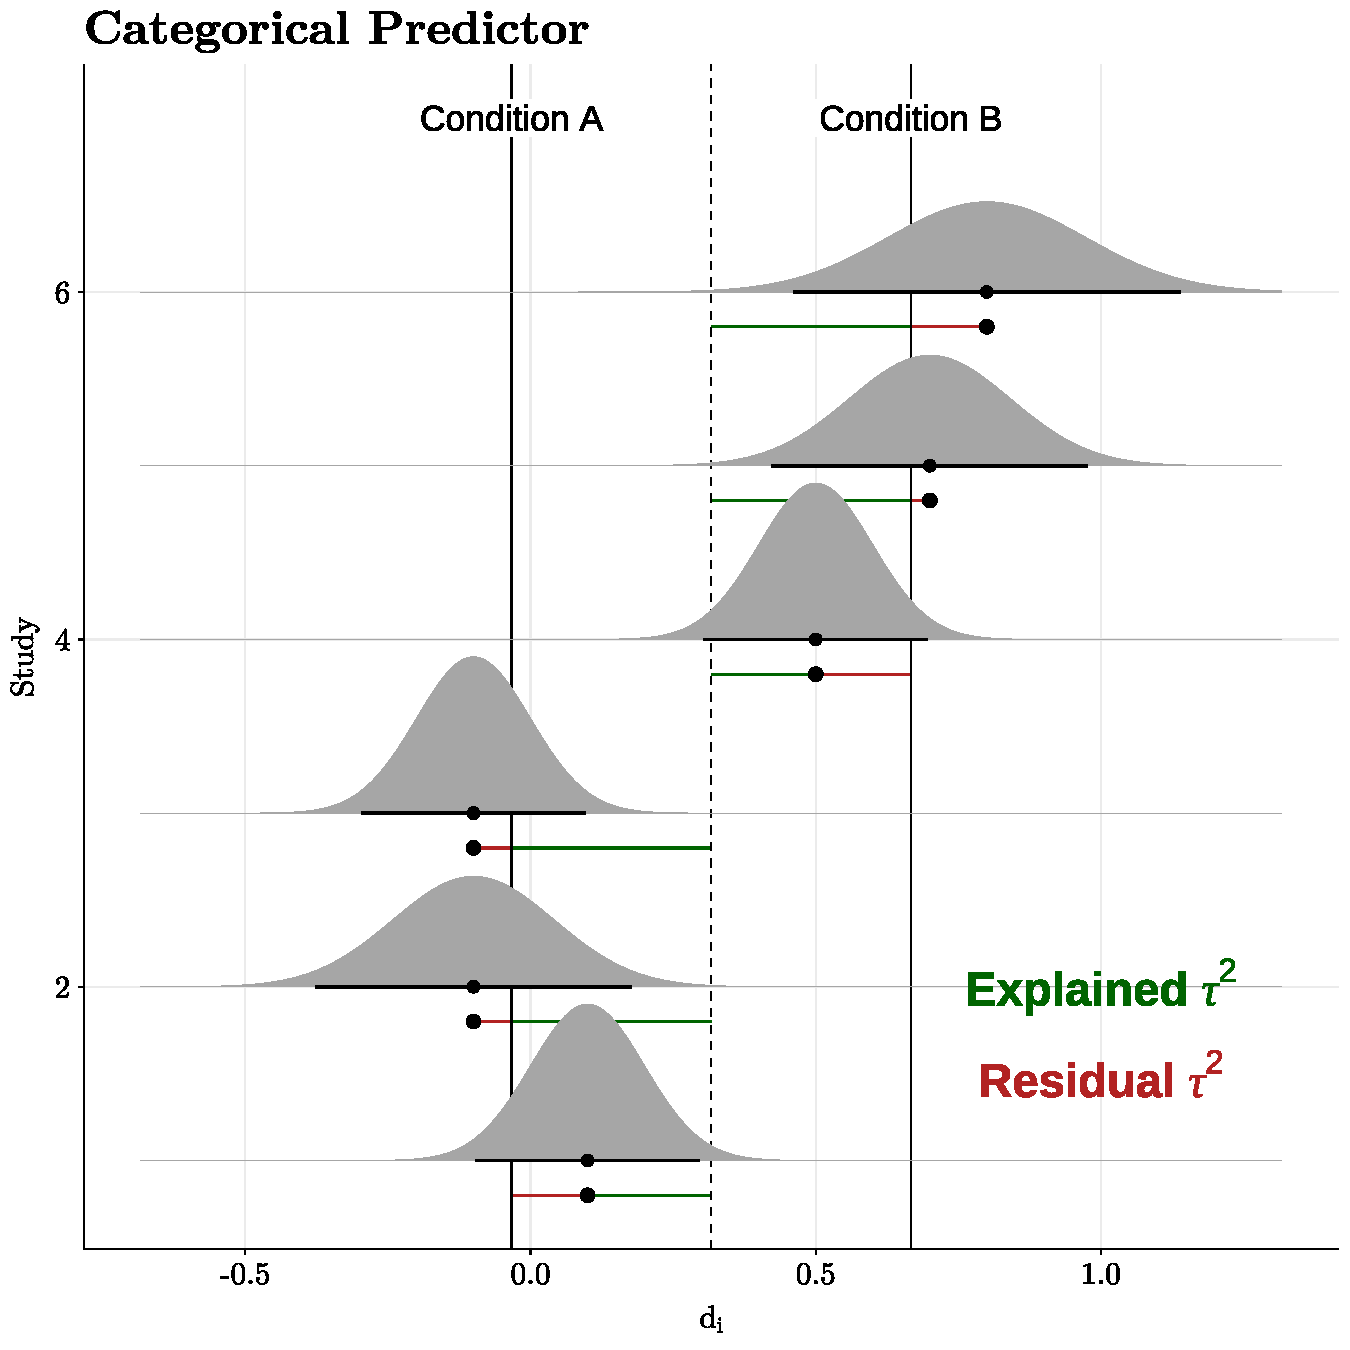
\includegraphics[width=0.8\linewidth]{paper_files/figure-latex/img-metaregression-bin-1} 

}

\caption{Graphical representation of a \emph{random-effects meta-regression} model with a categorical predictor (Condition A and Condition B). Each grey distribution represents the sampling distribution of included studies. The dotted line is the average effect (i.e., random-effects model without moderators). The effect size differs between conditions A and B, including the \emph{condition} moderator explaining part of the total heterogeneity (red plus green segments). The green segments depict the explained heterogeneity, and the red segments the residual (unexplained) heterogeneity.}\label{fig:img-metaregression-bin}
\end{figure}

\normalsize

\scriptsize

\begin{figure}[H]

{\centering 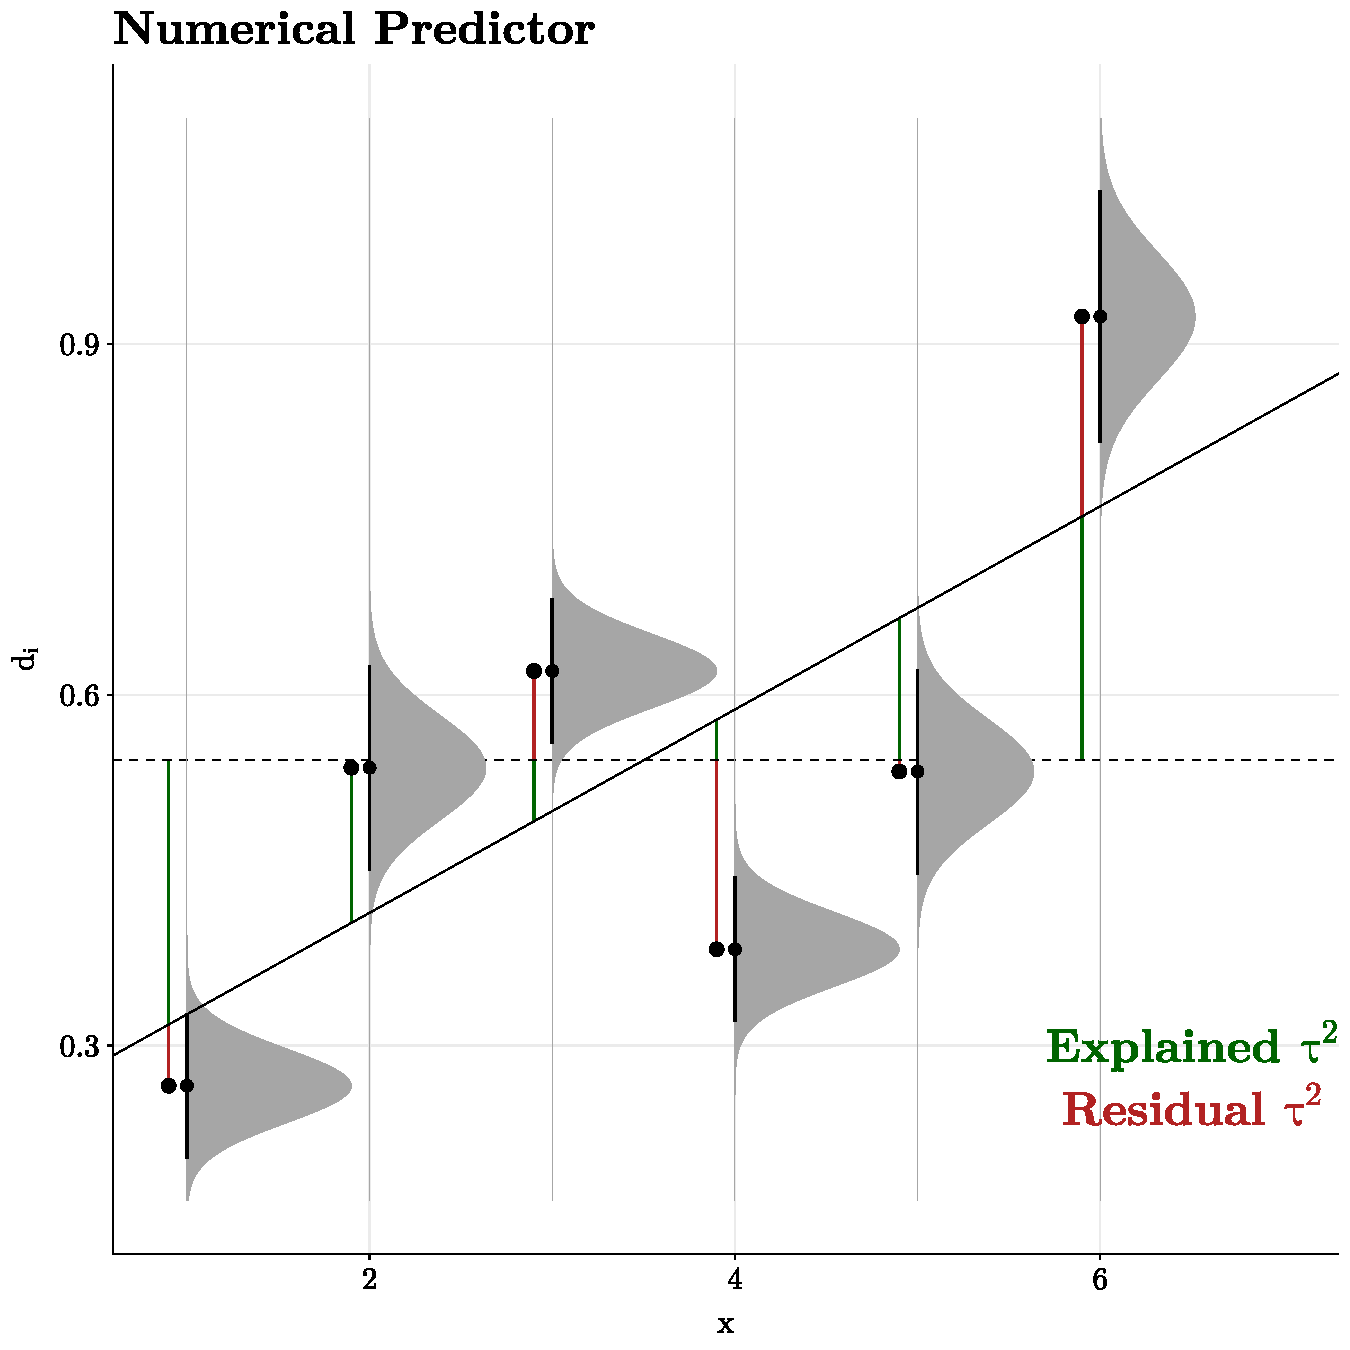
\includegraphics[width=0.8\linewidth]{paper_files/figure-latex/img-metaregression-num-1} 

}

\caption{Graphical representation of a \emph{random-effects meta-regression} model with a numerical predictor (\(x\)). Each grey distribution represents the sampling distribution of included studies. The dotted line is the average effect (i.e., random-effects model without moderators). The effect size increases as a function of the \(x\) variable. Therefore, including \(x\) as a predictor explains the
heterogeneity. The rest of the Figure follows the same logic as Figure \ref{fig:img-metaregression-bin}.}\label{fig:img-metaregression-num}
\end{figure}

\normalsize

\hypertarget{meta-regression-with-a-categorical-moderator}{%
\subsubsection{Meta-regression with a categorical moderator}\label{meta-regression-with-a-categorical-moderator}}

A common example of meta-regression is by including a categorical predictor, including information about study-level features. In our example, a group of studies uses an online memory task while others use a standard lab-based task. The Equation \eqref{eq:random-effect-model} can be easily extended for a meta-regression model by including a variable encoding the type of task (online vs.~lab-based) and the expected difference between the two levels of the moderator (i.e., the \emph{lab vs.~online effect}). In regression terms, we could use a dummy variable (\(X_{1}\)) that takes the value of 0 for the \emph{lab-based task} (\emph{l}) and a value of 1 for an \emph{online task} (\emph{o})\footnote{The \emph{dummy coding} (also known as treatment coding) is the default in R and \texttt{metafor} but other coding schemes could be used (see Schad, Vasishth, Hohenstein, \& Kliegl, 2020 for an overview of contrast coding schemes)}. Now we fix \(\beta_{1}\) to be the \emph{lab vs.~online effect} Equation \eqref{eq:random-effect-model} into Equation \eqref{eq:meta-regression}. Now the product between \(\beta_{1}X_{1}\) will consider the \emph{lab vs.~online effect}. To simulate this meta-regression, we need to fix the \(\beta_{1}\) effect. Due to the fact that we are on a standardized scale, we can fix \(\beta_{1}\) to be the expected difference in Cohen's \(d\) scale between the two groups of studies. Crucially, despite \(\tau^{2}\) is still the heterogeneity between effect sizes, now we need to fix \(\tau^{2}\) considering that we included a moderator. In other terms, \(\tau_{r}^{2}\) is the residual heterogeneity after explaining the
variance due to \(X_{1}\). We can describe our model using two equations according to the value of \(X_{1}\) as reported in Equation \eqref{eq:meta-regression-equations}.

\begin{align}
\begin{gathered}
d_i = \beta_0 + \theta_i + \beta_1 X_1 + \epsilon_i \\
\theta_i \sim \mathcal{N}(0, \tau^2) \\
\epsilon_i \sim \mathcal{N}(0,\sigma^2_i)
\label{eq:meta-regression}
\end{gathered}
\end{align}

\begin{align}
\begin{gathered}
d_i = \beta_0 + \theta_i + \beta_1 X_1 + \epsilon_i \\
d_{il} = \beta_0 + \theta_i + \beta_1 \times 0 + \epsilon_i \\
d_{io} = \beta_0 + \theta_i + \beta_1 \times 1 + \epsilon_i \\
\label{eq:meta-regression-equations}
\end{gathered}
\end{align}

We can simulate the same scenario of the random-effects model with \(k_o = 15\) (\emph{online tasks}) and \(k_l = 15\) (\emph{lab-based tasks}). Then we fix the \(\beta_1 = 0.2\) and \(\tau_r^2 = 0.1\) (\(r\) for residual).

\scriptsize

\begin{Shaded}
\begin{Highlighting}[]
\FunctionTok{set.seed}\NormalTok{(seed)}
\NormalTok{k }\OtherTok{\textless{}{-}} \DecValTok{30} \CommentTok{\# the total number of studies}
\NormalTok{b0 }\OtherTok{\textless{}{-}} \FloatTok{0.1} \CommentTok{\# intercept, the effect size of the lab{-}based studies}
\NormalTok{b1 }\OtherTok{\textless{}{-}} \FloatTok{0.2} \CommentTok{\# the difference between the two levels of the moderator}
\NormalTok{tau2r }\OtherTok{\textless{}{-}} \FloatTok{0.1} \CommentTok{\# the residual heterogeneity}
\NormalTok{n }\OtherTok{\textless{}{-}} \DecValTok{30} \CommentTok{\# the sample size per group, per study}

\NormalTok{sim }\OtherTok{\textless{}{-}} \FunctionTok{make\_data}\NormalTok{(}\AttributeTok{k =}\NormalTok{ k, }\AttributeTok{nc =}\NormalTok{ n, }\AttributeTok{nt =}\NormalTok{ n, }\AttributeTok{exp =} \FunctionTok{rep}\NormalTok{(}\FunctionTok{c}\NormalTok{(}\StringTok{"lab"}\NormalTok{, }\StringTok{"online"}\NormalTok{), }\AttributeTok{each =}\NormalTok{ k}\SpecialCharTok{/}\DecValTok{2}\NormalTok{))}

\NormalTok{sim}\SpecialCharTok{$}\NormalTok{theta\_i }\OtherTok{\textless{}{-}} \FunctionTok{rnorm}\NormalTok{(k, }\DecValTok{0}\NormalTok{, }\FunctionTok{sqrt}\NormalTok{(tau2r)) }\CommentTok{\# the by{-}study residual adjustment}
\NormalTok{sim}\SpecialCharTok{$}\NormalTok{b0\_theta\_i\_x }\OtherTok{\textless{}{-}}\NormalTok{ b0 }\SpecialCharTok{+}\NormalTok{ sim}\SpecialCharTok{$}\NormalTok{theta\_i }\SpecialCharTok{+}\NormalTok{ b1}\SpecialCharTok{*}\FunctionTok{ifelse}\NormalTok{(sim}\SpecialCharTok{$}\NormalTok{exp }\SpecialCharTok{==} \StringTok{"lab"}\NormalTok{, }\DecValTok{0}\NormalTok{, }\DecValTok{1}\NormalTok{)}

\NormalTok{sim }\OtherTok{\textless{}{-}} \FunctionTok{sim\_studies}\NormalTok{(sim}\SpecialCharTok{$}\NormalTok{b0\_theta\_i\_x, sim}\SpecialCharTok{$}\NormalTok{nc, sim}\SpecialCharTok{$}\NormalTok{nt, }\AttributeTok{data =}\NormalTok{ sim)}
\NormalTok{res }\OtherTok{\textless{}{-}} \FunctionTok{rma}\NormalTok{(yi, vi, }\AttributeTok{mods =} \SpecialCharTok{\textasciitilde{}}\NormalTok{exp, }\AttributeTok{method =} \StringTok{"REML"}\NormalTok{, }\AttributeTok{data =}\NormalTok{ sim)}
\end{Highlighting}
\end{Shaded}

\normalsize

Now we can fit the meta-regression model with the \texttt{rma} function as for the random-effects model with the addition of \texttt{mods\ =\ \textasciitilde{}\ exp} that indicates which variable/s to consider as moderators. The results are presented in Table \ref{tab:res-meta-reg-dummy}. Now the model will estimate an \emph{intercept} parameter (i.e., \(\beta_0\)) that is the value of \(y\) when \(X_1\) is zero (i.e., for lab-based studies) or in other terms the expected value for lab-based studies. Then the \(\beta_1\) parameter represents the estimated difference in \(y\) between the values of \(X_1\) (i.e., lab-based vs online experiments). As said before, \(\tau^2\) is now the residual heterogeneity that is interpreted as the variability between effect sizes after controlling for the moderator \(X_1\).

Now we can fit the meta-regression model with the \texttt{rma} function as for the random-effects model with the addition of mods = \texttt{\textasciitilde{}\ exp} that indicates which variable/s to consider as moderators. The results are presented in Table \ref{tab:res-meta-reg-dummy}. Next, the model will estimate an \emph{intercept} parameter (i.e., \(\beta_{0}\)) that is the value of \(y\) when \(X_{1}\) is zero (i.e., for lab-based studies) or, in other terms, the expected value for lab-based studies. Then the \(\beta_{1}\) parameter represents the estimated difference in \(y\) between the values of \(X_{1}\) (i.e., lab-based vs.~online experiments). As mentioned above, \(\tau^{2}\) the residual heterogeneity is now interpreted as the variability between effect sizes after controlling for the moderator \(X_{1}\).

\scriptsize

\begin{table}[H]

\caption{\label{tab:res-meta-reg-dummy}Summary of the \emph{random-effect} model with a categorical predictor (lab vs online experiments). The \texttt{intercept} is the average effect for lab-based experiments and \texttt{exponline} is the difference between lab-based and online experiments. The \(R^2\) is the percentage of explained heterogeneity and \(\tau^2_r\) is the estimated residual heterogeneity. Other parameters are the same as the standard \emph{random-effect} model (see Table \ref{tab:res-random-effect}).}
\centering
\fontsize{9}{11}\selectfont
\begin{tabular}[t]{ccccc}
\toprule
 & $\beta$ & 95\% CI & z & p\\
\midrule
intercept & 0.041 (SE = 0.101) & $[-0.157, 0.238]$ & 0.403 & 0.687\\
exponline & 0.321 (SE = 0.143) & $[0.040, 0.601]$ & 2.243 & 0.025\\
\bottomrule
\multicolumn{5}{l}{\textsuperscript{} $k = 30$}\\
\multicolumn{5}{l}{\textsuperscript{} $\tau^2_r = 0.085$ ($SE = 0.041$)}\\
\multicolumn{5}{l}{\textsuperscript{} $R^2 = 19.902\%$}\\
\multicolumn{5}{l}{\textsuperscript{} $I^2 = 55.435\%$}\\
\end{tabular}
\end{table}

\normalsize

\hypertarget{meta-regression-with-a-numerical-moderator}{%
\subsubsection{Meta-regression with a numerical moderator}\label{meta-regression-with-a-numerical-moderator}}

The same approach can be used for a continuous predictor. For example, we can simulate that the average participant's age within each study could explain part of the observed heterogeneity. Now the \(X_1\) is a continuous predictor representing the average age for each study and \(\beta_1\) is the effect size increase for a unit increase (i.e., 1 year) of average age. Sometimes guessing a plausible \(\beta_1\) value with a continuous predictor is not straightforward. A first strategy could be to use values estimated from the literature. Another approach consists in setting up the model and simulating several expected \(d_i\) and calculating the range of simulated values. A third possibility is fixing the proportion of explained heterogeneity calculating the \(\beta_1\) value accordingly. As in standard regression analysis, we can use the \(R^2\) statistic to describe the amount of heterogeneity explained by the included moderators. Equation \eqref{eq:rsquared} reports how to calculate the \(R^2\) for a meta-regression model. The \(\tau^2_{r}\) is the residual heterogeneity after considering the moderators and \(\tau^2_{f}\) is the heterogeneity estimated without considering the moderators. In the next sections, we will present an example of the simulation-based and the \(R^2\) based approaches.

\begin{align}
\begin{aligned}
R^2 = 1 - \frac{\tau^2_{r}}{\tau^2_{f}}
\label{eq:rsquared}
\end{aligned}
\end{align}

In terms of regression parameters now the intercept (\(\beta_0\)) is no longer the overall effect or the average of one category as in the previous example but the estimated value for a specific \(X_1\) thus for a specific age. If \(X_1\) is a variable representing the average age for each study, then the \(\beta_0\) is the average effect size when the age is zero. Depending on the moderator, the intercept is interpreted in different ways. For example, with the age, the intercept has no empirical meaning given that no studies could have a participant average age of zero. A strategy could be to mean-center the age (i.e., subtracting from each study age the average age across the study). Now the intercept is still the average effect size when the age is zero but now zero is the average age. Importantly, the contrast coding for categorical predictors or centering numerical variables does not affect the overall model estimation but only parameters values and interpretation.

\hypertarget{assessing-the-impact-of-beta_1}{%
\paragraph{\texorpdfstring{Assessing the impact of \(\beta_1\)}{Assessing the impact of \textbackslash beta\_1}}\label{assessing-the-impact-of-beta_1}}

As reported in the previous section, a strategy to guess plausible values for \(\beta_{1}\) is by simulating several expected \(y_{i}\) given the meta-regression equation and summarizing or plotting the effect size range. The range of simulated \(y_{i}\) values are also affected by the simulated age values across studies. However, it is probably more intuitive to guess a plausible range of moderator values compared to the \(\beta_{1}\) value. In this specific example, if all studies target a specific population (e.g., adults below 50 years), the expected average age range can be easily simulated. In our case, we simulated \(k\) average age values from a uniform distribution \(\text{ag}e_{i} \sim U\left( 20,40 \right)\). Then we can plot the distribution of \(d_{i}\) values to check the plausibility of simulated values. As shown in Figure \ref{fig:plot-meta-reg-plausible-implausible}, with the same range for the moderator, a \(\beta_{1} = 0.1\) gives a plausible effect sizes range while a \(\beta_{1} = 0.7\) predicts very extreme values.

\scriptsize

\begin{Shaded}
\begin{Highlighting}[]
\FunctionTok{set.seed}\NormalTok{(seed)}
\NormalTok{k }\OtherTok{\textless{}{-}} \DecValTok{1000} \CommentTok{\# number of studies}
\NormalTok{b0 }\OtherTok{\textless{}{-}} \FloatTok{0.3} \CommentTok{\# the intercept i.e., average yi when x is 0}
\NormalTok{b1 }\OtherTok{\textless{}{-}} \FunctionTok{c}\NormalTok{(}\FloatTok{0.1}\NormalTok{, }\FloatTok{0.7}\NormalTok{) }\CommentTok{\# the beta1 i.e., the increase in yi for an increase in 1 year}
\NormalTok{tau2r }\OtherTok{\textless{}{-}} \FloatTok{0.1} \CommentTok{\# the residual heterogeneity after including x1}
\NormalTok{n }\OtherTok{\textless{}{-}} \DecValTok{30} \CommentTok{\# number of participants per study, per group}
\NormalTok{x1 }\OtherTok{\textless{}{-}} \FunctionTok{runif}\NormalTok{(k, }\DecValTok{20}\NormalTok{, }\DecValTok{40}\NormalTok{) }\CommentTok{\# random mean{-}age for each study}
\NormalTok{x10 }\OtherTok{\textless{}{-}}\NormalTok{ x1 }\SpecialCharTok{{-}} \FunctionTok{mean}\NormalTok{(x1) }\CommentTok{\# centering the age}

\NormalTok{sim }\OtherTok{\textless{}{-}}\NormalTok{ tidyr}\SpecialCharTok{::}\FunctionTok{expand\_grid}\NormalTok{(}\AttributeTok{id =} \DecValTok{1}\SpecialCharTok{:}\NormalTok{k, }\AttributeTok{nc =}\NormalTok{ n, }\AttributeTok{nt =}\NormalTok{ n, }\AttributeTok{b1 =}\NormalTok{ b1)}

\NormalTok{sim}\SpecialCharTok{$}\NormalTok{age }\OtherTok{\textless{}{-}} \FunctionTok{rep}\NormalTok{(x1, }\AttributeTok{each =} \DecValTok{2}\NormalTok{)}
\NormalTok{sim}\SpecialCharTok{$}\NormalTok{age0 }\OtherTok{\textless{}{-}} \FunctionTok{rep}\NormalTok{(x10, }\AttributeTok{each =} \DecValTok{2}\NormalTok{)}

\NormalTok{theta\_i }\OtherTok{\textless{}{-}} \FunctionTok{rnorm}\NormalTok{(k, }\DecValTok{0}\NormalTok{, }\FunctionTok{sqrt}\NormalTok{(tau2r))}
\NormalTok{sim}\SpecialCharTok{$}\NormalTok{theta\_i }\OtherTok{\textless{}{-}} \FunctionTok{rep}\NormalTok{(theta\_i, }\AttributeTok{each =} \DecValTok{2}\NormalTok{)}

\NormalTok{sim}\SpecialCharTok{$}\NormalTok{b0\_theta\_i\_x }\OtherTok{\textless{}{-}}\NormalTok{ b0 }\SpecialCharTok{+}\NormalTok{ sim}\SpecialCharTok{$}\NormalTok{theta\_i }\SpecialCharTok{+}\NormalTok{ sim}\SpecialCharTok{$}\NormalTok{b1}\SpecialCharTok{*}\NormalTok{sim}\SpecialCharTok{$}\NormalTok{age0}

\NormalTok{sim }\OtherTok{\textless{}{-}} \FunctionTok{sim\_studies}\NormalTok{(sim}\SpecialCharTok{$}\NormalTok{b0\_theta\_i\_x, sim}\SpecialCharTok{$}\NormalTok{nc, sim}\SpecialCharTok{$}\NormalTok{nt, }\AttributeTok{data =}\NormalTok{ sim)}
\end{Highlighting}
\end{Shaded}

\normalsize

\scriptsize

\begin{figure}[H]

{\centering 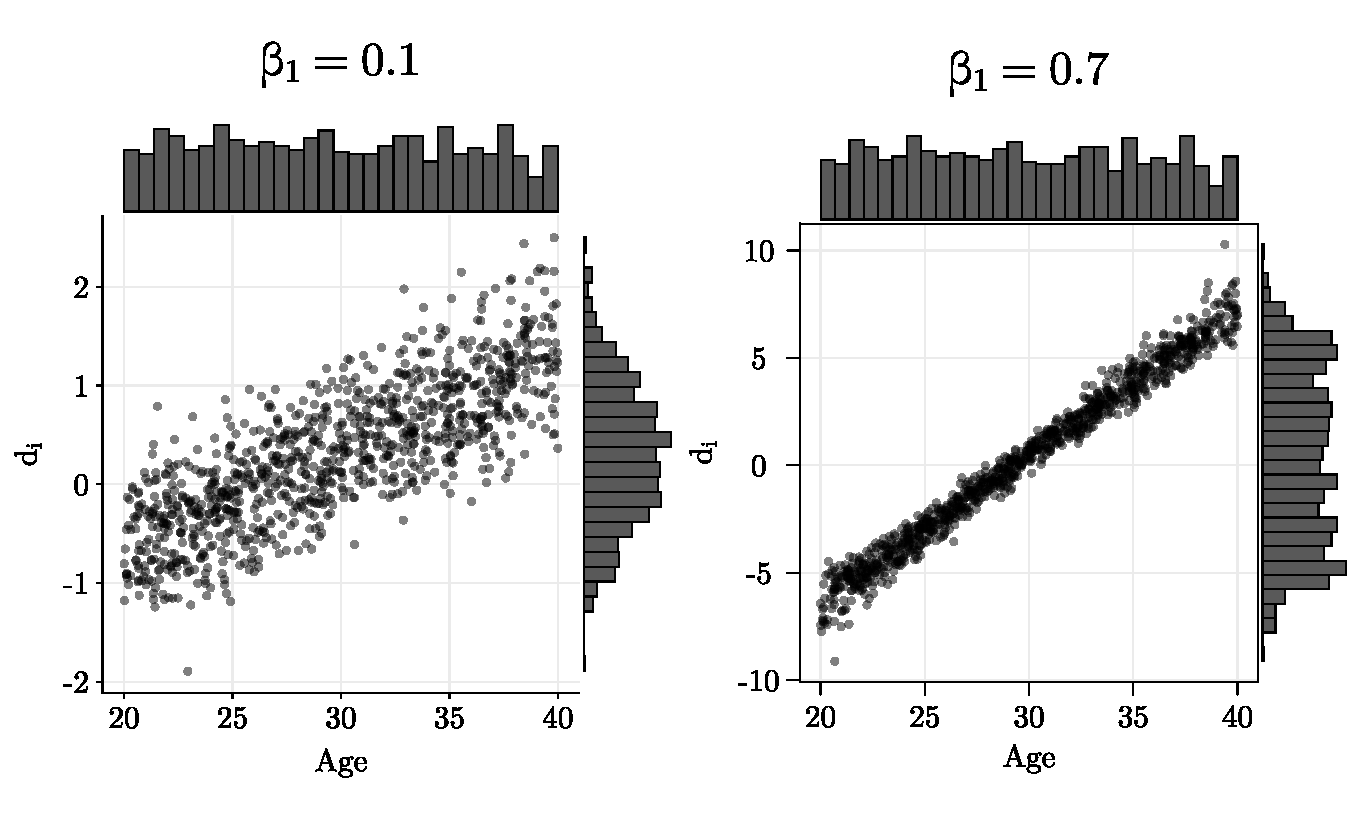
\includegraphics[width=0.8\linewidth]{paper_files/figure-latex/plot-meta-reg-plausible-implausible-1} 

}

\caption{Scatter plots with marginal histograms for the range of simulated \(d_i\) with two \(\beta_1\) values. The x-axis depicts the average age of simulated studies and the y-axis depicts the simulated effect size. On the left, the majority of simulated values range between -1.5 and 1.5 thus \(\beta_1 = 0.1\) can be considered a plausible value. On the right, (\(\beta = 0.7\)) values range between -10 to 10 that despite theoretically possible is highly implausible values in real meta-analysis for psychological data.}\label{fig:plot-meta-reg-plausible-implausible}
\end{figure}

\normalsize

\hypertarget{simulating-using-r2}{%
\paragraph{\texorpdfstring{Simulating using \(R^2\)}{Simulating using R\^{}2}}\label{simulating-using-r2}}

A more intuitive way to simulate a continuous predictor is fixing the desired \(R^{2}\) value and finding the coefficient that produces the desired value. This approach has been implemented by Lopez-Lopez and colleagues (2014). We can use Equation \eqref{eq:beta-from-r2} to find the \(\beta_{1}\) value that is associated with a certain \(R^{2}\).

\begin{align}
\begin{aligned}
\beta^2_1 = \tau^2R^2 \\
\tau^2_{r} = \tau^2 - \beta^2_1
\label{eq:beta-from-r2}
\end{aligned}
\end{align}

Now we can simulate the regression model using \(\sqrt{\beta^2_1}\) as coefficient and \(\tau_{r}^{2}\) as residual heterogeneity. Results from the fitted model fixing the \(R^{2}\) values are presented in Table \ref{tab:res-meta-reg-numerical-r2} and Figure \ref{fig:plot-meta-reg-numerical-r2}. As Lopez-Lopez and colleagues (2014) demonstrated, to reliably estimate \(R^{2}\) the number of studies needs to be large\footnote{see also \url{https://www.metafor-project.org/doku.php/tips:ci_for_r2} for a discussion about confidence intervals for the \(R^2\) statistic}. Lopez-Lopez and colleagues (2014) generated the moderator (\(X_{1}\)) values from a standard normal distribution. In the following example, we standardized the moderator (\texttt{scale()}) after simulating values on the \emph{age} scale
(e.g., \texttt{runif(k,\ 20,\ 40)}).

\scriptsize

\begin{Shaded}
\begin{Highlighting}[]
\FunctionTok{set.seed}\NormalTok{(seed)}
\NormalTok{k }\OtherTok{\textless{}{-}} \DecValTok{100} \CommentTok{\# the number of studies}
\NormalTok{r2 }\OtherTok{\textless{}{-}} \FloatTok{0.2} \CommentTok{\# the desired r2 value}
\NormalTok{tau2 }\OtherTok{\textless{}{-}} \FloatTok{0.3} \CommentTok{\# the overall tau2}
\NormalTok{b0 }\OtherTok{\textless{}{-}} \FloatTok{0.3} \CommentTok{\# the intercept i.e., average yi when x1 is 0}
\NormalTok{b1\_2 }\OtherTok{\textless{}{-}}\NormalTok{ tau2 }\SpecialCharTok{*}\NormalTok{ r2 }\CommentTok{\# the beta1\^{}2 i.e., the increase in yi for an increase in 1 year}
\NormalTok{b1 }\OtherTok{\textless{}{-}} \FunctionTok{sqrt}\NormalTok{(b1\_2) }\CommentTok{\# b1\_2 is squared, back to the original scale}
\NormalTok{tau2r }\OtherTok{\textless{}{-}}\NormalTok{ tau2 }\SpecialCharTok{{-}}\NormalTok{ b1\_2 }\CommentTok{\# the residual heterogeneity after including x1}
\NormalTok{n }\OtherTok{\textless{}{-}} \DecValTok{30} \CommentTok{\# number of participants per study, per group}
\NormalTok{x1 }\OtherTok{\textless{}{-}} \FunctionTok{runif}\NormalTok{(k, }\DecValTok{20}\NormalTok{, }\DecValTok{40}\NormalTok{) }\CommentTok{\# random mean{-}age for each study}

\NormalTok{sim }\OtherTok{\textless{}{-}} \FunctionTok{make\_data}\NormalTok{(}\AttributeTok{k =}\NormalTok{ k, }\AttributeTok{nt =}\NormalTok{ n, }\AttributeTok{nc =}\NormalTok{ n, }\AttributeTok{age =}\NormalTok{ x1)}

\NormalTok{sim}\SpecialCharTok{$}\NormalTok{theta\_i }\OtherTok{\textless{}{-}} \FunctionTok{rnorm}\NormalTok{(k, }\DecValTok{0}\NormalTok{, }\FunctionTok{sqrt}\NormalTok{(tau2r))}
\NormalTok{sim}\SpecialCharTok{$}\NormalTok{age0 }\OtherTok{\textless{}{-}} \FunctionTok{scale}\NormalTok{(sim}\SpecialCharTok{$}\NormalTok{age, }\AttributeTok{center =} \ConstantTok{TRUE}\NormalTok{, }\AttributeTok{scale =} \ConstantTok{TRUE}\NormalTok{) }\CommentTok{\# standardize the moderator}
\NormalTok{sim}\SpecialCharTok{$}\NormalTok{b0\_theta\_i\_x }\OtherTok{\textless{}{-}}\NormalTok{ b0 }\SpecialCharTok{+}\NormalTok{ sim}\SpecialCharTok{$}\NormalTok{theta\_i }\SpecialCharTok{+}\NormalTok{ b1}\SpecialCharTok{*}\NormalTok{sim}\SpecialCharTok{$}\NormalTok{age0}

\NormalTok{sim }\OtherTok{\textless{}{-}} \FunctionTok{sim\_studies}\NormalTok{(sim}\SpecialCharTok{$}\NormalTok{b0\_theta\_i\_x, sim}\SpecialCharTok{$}\NormalTok{nt, sim}\SpecialCharTok{$}\NormalTok{nc, }\AttributeTok{data =}\NormalTok{ sim)}
\NormalTok{res }\OtherTok{\textless{}{-}} \FunctionTok{rma}\NormalTok{(yi, vi, }\AttributeTok{mods =} \SpecialCharTok{\textasciitilde{}}\NormalTok{age0, }\AttributeTok{method =} \StringTok{"REML"}\NormalTok{, }\AttributeTok{data =}\NormalTok{ sim)}
\end{Highlighting}
\end{Shaded}

\normalsize

\scriptsize

\begin{table}[H]

\caption{\label{tab:res-meta-reg-numerical-r2}Summary of the \emph{random-effects} model fixing the \(R^{2}\) value. The \texttt{intercept} is the effect size for the average \texttt{age} (given that age is mean-centered). The \texttt{age0} parameter is the slope between \texttt{age} and the effect size interpreted as an increase in effect size for a unit increase in the average age. Other parameters are the same as described in Table \ref{tab:res-random-effect} and \ref{tab:res-meta-reg-dummy}.}
\centering
\fontsize{9}{11}\selectfont
\begin{tabular}[t]{ccccc}
\toprule
 & $\beta$ & 95\% CI & z & p\\
\midrule
intercept & 0.335 (SE = 0.051) & $[0.236, 0.435]$ & 6.586 & < 0.001\\
age0 & 0.163 (SE = 0.051) & $[0.063, 0.263]$ & 3.184 & 0.001\\
\bottomrule
\multicolumn{5}{l}{\textsuperscript{} $k = 100$}\\
\multicolumn{5}{l}{\textsuperscript{} $\tau^2_r = 0.189$ ($SE = 0.037$)}\\
\multicolumn{5}{l}{\textsuperscript{} $R^2 = 11.283\%$}\\
\multicolumn{5}{l}{\textsuperscript{} $I^2 = 73.038\%$}\\
\end{tabular}
\end{table}

\normalsize

\scriptsize

\begin{figure}[H]

{\centering 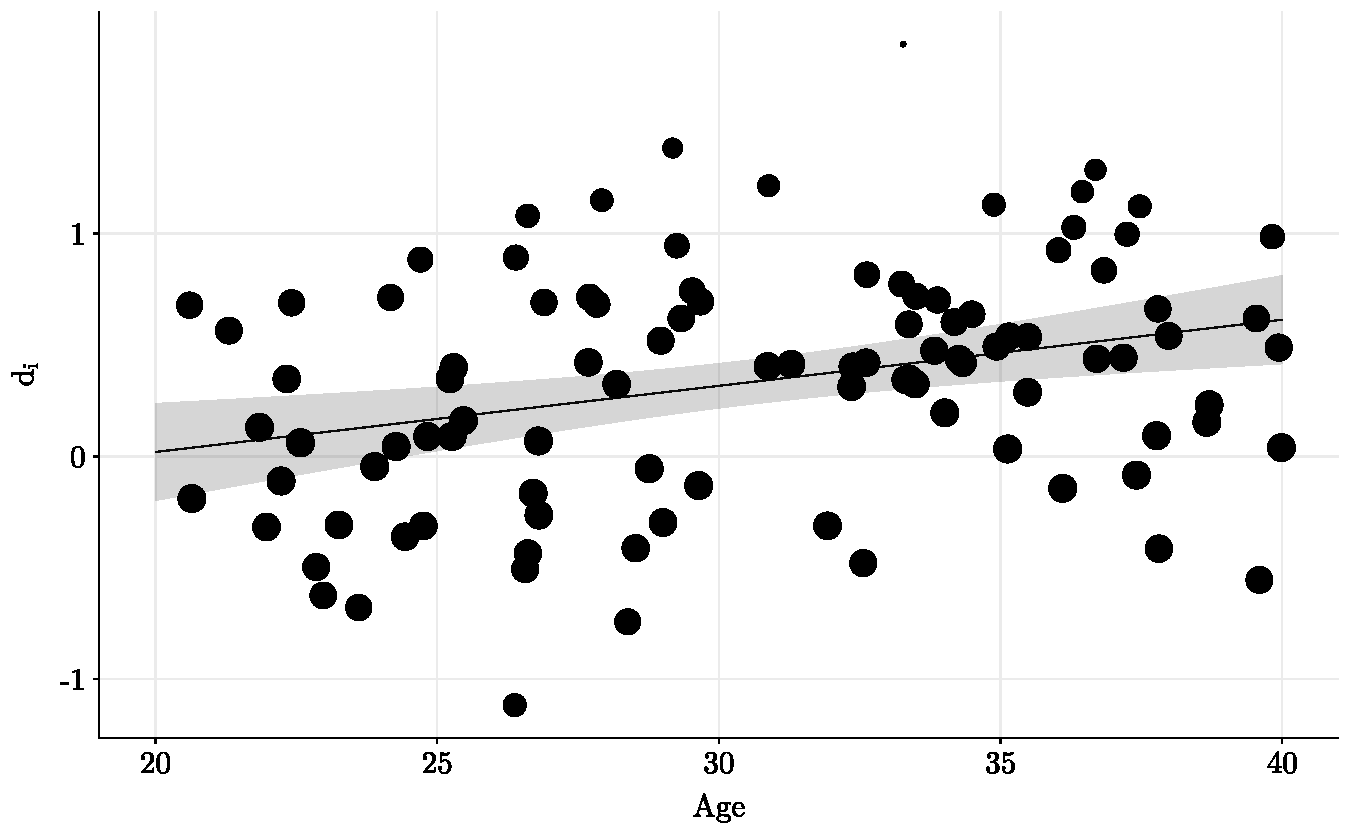
\includegraphics[width=0.8\linewidth]{paper_files/figure-latex/plot-meta-reg-numerical-r2-1} 

}

\caption{Meta-regression results for the \emph{random-effects model} with a numerical moderator. Each effect size is represented with a black dot where the dimension represents the weight according to the inverse of the precision. The line represents the estimated meta-regression slope with the 95\% confidence interval (grey bands).}\label{fig:plot-meta-reg-numerical-r2}
\end{figure}

\normalsize

\hypertarget{power-analysis}{%
\section{Power Analysis}\label{power-analysis}}

The previous simulation examples can be easily implemented for multiple purposes. For example, we can use different effect sizes and variance estimators when using the \texttt{sim\_study()} function to check the impact on the fitted meta-analysis model. However, one of the most critical applications is estimating the power of a specific statistical model.

As explained in the introduction, there are several approaches and tools to estimate the power of \emph{fixed} and \emph{random-effects models} (see Borenstein et al., 2009, Chapter 29; Harrer, Cuijpers, \& Ebert, 2019, Chapter 14). These methods are easy to implement but made strong assumptions, such as the homogeneity of sample size, and did not consider the uncertainty in estimating \(\tau^{2}\). Jackson and colleagues (2017)
partially solve the issue by developing an interesting method that takes into account the uncertainty in estimating \(\tau^{2}\) without using simulations. However, only Monte Carlo simulations can consider complex scenarios and extra parameters.

A general Monte Carlo simulation for the power analysis can be implemented with the following steps:

\begin{enumerate}
\def\labelenumi{\arabic{enumi}.}
\tightlist
\item
  Choose the model that generates the data (e.g., fixed, or random-effects model).
\item
  Fix the relevant parameters (e.g., \(\tau^{2}\) and \(\theta\)).
\item
  Simulate a dataset.
\item
  Fit the appropriate model.
\item
  Store the p-value associated with the parameter of interest
\item
  Repeat 3-5 a large number of times (e.g., 10000).
\item
  Calculate the power as the proportion of p-values below the \(\alpha\) level.
\end{enumerate}

For example, we can estimate the power of a \emph{random-effects model} by repeating the simulation presented in Section \ref{re-model} many times. We simulated heterogeneity of sample sizes sampling \(n_{T}\) and \(n_{C}\) values from a Poisson distribution with \(\lambda = 20\). In this way, on average, the sample size is 20 for primary studies with a certain amount of heterogeneity. Usually, it is more informative to simulate different scenarios according to the relevant parameters, such as sample sizes, number of studies, or heterogeneity. For example, we can estimate the power with a different number of studies \(k\). We define the \texttt{do\_sim()} function that, according to the input parameter, repeats the simulation a certain number of times (i.e., \texttt{nsim})\footnote{We are using the \texttt{purrr::pmap()} function that can be considered very similar to \texttt{mapply()} but less verbose. Compared to \texttt{mapply()}, the \texttt{sim\_grid} columns are directly passed to the \texttt{do\_sim()} function without specifying the order.}. Increasing the number of simulations will increase the power analysis estimation precision. Then the \texttt{summary\_sim()} function analyzes each simulation returning the relevant values. We repeat the simulation of the \emph{random-effects model} several times with different parameters.

\scriptsize

\begin{Shaded}
\begin{Highlighting}[]

\NormalTok{do\_sim }\OtherTok{\textless{}{-}} \ControlFlowTok{function}\NormalTok{(k, theta, tau2, navg, nmin, nsim, }\AttributeTok{alpha =} \FloatTok{0.05}\NormalTok{, }\AttributeTok{summary =} \ConstantTok{TRUE}\NormalTok{)\{}
  \CommentTok{\# preallocate for computation speed}
\NormalTok{  p }\OtherTok{\textless{}{-}} \FunctionTok{vector}\NormalTok{(}\AttributeTok{mode =} \StringTok{"numeric"}\NormalTok{, }\AttributeTok{length =}\NormalTok{ nsim)}
  
  \CommentTok{\# start the simulation loop}
  \ControlFlowTok{for}\NormalTok{(i }\ControlFlowTok{in} \DecValTok{1}\SpecialCharTok{:}\NormalTok{nsim)\{}
\NormalTok{    theta\_i }\OtherTok{\textless{}{-}} \FunctionTok{rnorm}\NormalTok{(k, }\DecValTok{0}\NormalTok{, }\FunctionTok{sqrt}\NormalTok{(tau2))}
\NormalTok{    theta\_theta\_i }\OtherTok{\textless{}{-}}\NormalTok{ theta }\SpecialCharTok{+}\NormalTok{ theta\_i}
    \CommentTok{\# simulate sample size}
\NormalTok{    n }\OtherTok{\textless{}{-}}\NormalTok{ nmin }\SpecialCharTok{+} \FunctionTok{rpois}\NormalTok{(k, navg }\SpecialCharTok{{-}}\NormalTok{ nmin)}
    \CommentTok{\# simulate the studies}
\NormalTok{    sim }\OtherTok{\textless{}{-}} \FunctionTok{sim\_studies}\NormalTok{(theta\_theta\_i, n, n, }\AttributeTok{data =} \ConstantTok{NULL}\NormalTok{)}
\NormalTok{    res }\OtherTok{\textless{}{-}} \FunctionTok{rma}\NormalTok{(yi, vi, }\AttributeTok{method =} \StringTok{"REML"}\NormalTok{, }\AttributeTok{data =}\NormalTok{ sim)}
\NormalTok{    p[i] }\OtherTok{\textless{}{-}}\NormalTok{ res}\SpecialCharTok{$}\NormalTok{pval }\CommentTok{\# store the p value}
\NormalTok{  \}}
  \ControlFlowTok{if}\NormalTok{(summary)\{}
    \CommentTok{\# return directly the power}
    \FunctionTok{summary\_sim}\NormalTok{(p, alpha)}
\NormalTok{  \}}\ControlFlowTok{else}\NormalTok{\{}
    \CommentTok{\# return the list of pvalues}
    \FunctionTok{data.frame}\NormalTok{(p)}
\NormalTok{  \}}
\NormalTok{\}}

\NormalTok{summary\_sim }\OtherTok{\textless{}{-}} \ControlFlowTok{function}\NormalTok{(p, alpha)\{}
\NormalTok{  power }\OtherTok{\textless{}{-}} \FunctionTok{mean}\NormalTok{(p }\SpecialCharTok{\textless{}=}\NormalTok{ alpha) }\CommentTok{\# compute power}
  \FunctionTok{data.frame}\NormalTok{(power)}
\NormalTok{\}}
\end{Highlighting}
\end{Shaded}

\normalsize

Simulation results are presented in Figure \ref{fig:plot-power-analysis} and Table \ref{tab:tab-power-analysis-example} showing that to reach 80\% power (usually considered an appropriate level) with \(\alpha = 0.05\) we need \textasciitilde35 studies. The same approach could be used to estimate the power of a meta-regression by simply modifying the \texttt{do\_sim()} function simulating the effect of a moderator and extracting the relevant p-value.

\scriptsize

\begin{Shaded}
\begin{Highlighting}[]
\FunctionTok{set.seed}\NormalTok{(seed)}
\NormalTok{nsim }\OtherTok{\textless{}{-}} \DecValTok{5000} \CommentTok{\# number of simulations per condition (5000, higher is better)}
\NormalTok{k }\OtherTok{\textless{}{-}} \FunctionTok{c}\NormalTok{(}\DecValTok{5}\NormalTok{, }\DecValTok{15}\NormalTok{, }\DecValTok{25}\NormalTok{, }\DecValTok{35}\NormalTok{, }\DecValTok{50}\NormalTok{) }\CommentTok{\# number of studies}
\NormalTok{theta }\OtherTok{\textless{}{-}} \FloatTok{0.3} \CommentTok{\# the average effect size}
\NormalTok{tau2 }\OtherTok{\textless{}{-}} \FloatTok{0.3} \CommentTok{\# the heterogeneity}
\NormalTok{navg }\OtherTok{\textless{}{-}} \DecValTok{20} \CommentTok{\# average sample size per study}
\NormalTok{nmin }\OtherTok{\textless{}{-}} \DecValTok{10} \CommentTok{\# minimum sample size per study}
\NormalTok{alpha }\OtherTok{\textless{}{-}} \FloatTok{0.05} \CommentTok{\# the alpha level}

\CommentTok{\# creating all combinations}
\NormalTok{sim\_grid }\OtherTok{\textless{}{-}}\NormalTok{ tidyr}\SpecialCharTok{::}\FunctionTok{expand\_grid}\NormalTok{(k, theta, tau2, navg, nmin, nsim)}

\CommentTok{\# apply the simulation to all combinations}
\NormalTok{res }\OtherTok{\textless{}{-}}\NormalTok{ purrr}\SpecialCharTok{::}\FunctionTok{pmap}\NormalTok{(sim\_grid, do\_sim)}

\CommentTok{\# combine the results}
\NormalTok{res }\OtherTok{\textless{}{-}}\NormalTok{ dplyr}\SpecialCharTok{::}\FunctionTok{bind\_rows}\NormalTok{(res)}
\NormalTok{sim\_grid }\OtherTok{\textless{}{-}} \FunctionTok{cbind}\NormalTok{(sim\_grid, res)}
\end{Highlighting}
\end{Shaded}

\normalsize

\scriptsize

\begin{table}[H]

\begin{center}
\begin{threeparttable}

\caption{\label{tab:tab-power-analysis-example}The results from the power analysis simulation. The table depicts the simulation parameters, the estimated power using the \texttt{summary\_sim()} function, and the average sample size (\(n\)) across the simulations.}

\small{

\begin{tabular}{lllllll}
\toprule
k & \multicolumn{1}{c}{$\theta$} & \multicolumn{1}{c}{$\tau^2$} & \multicolumn{1}{c}{$n_{avg}$} & \multicolumn{1}{c}{$n_{min}$} & \multicolumn{1}{c}{nsim} & \multicolumn{1}{c}{Power}\\
\midrule
5 & 0.30 & 0.30 & 20 & 10 & 5000 & 0.25\\
15 & 0.30 & 0.30 & 20 & 10 & 5000 & 0.46\\
25 & 0.30 & 0.30 & 20 & 10 & 5000 & 0.65\\
35 & 0.30 & 0.30 & 20 & 10 & 5000 & 0.79\\
50 & 0.30 & 0.30 & 20 & 10 & 5000 & 0.92\\
\bottomrule
\end{tabular}

}

\end{threeparttable}
\end{center}

\end{table}

\normalsize

\scriptsize

\begin{figure}[H]

{\centering 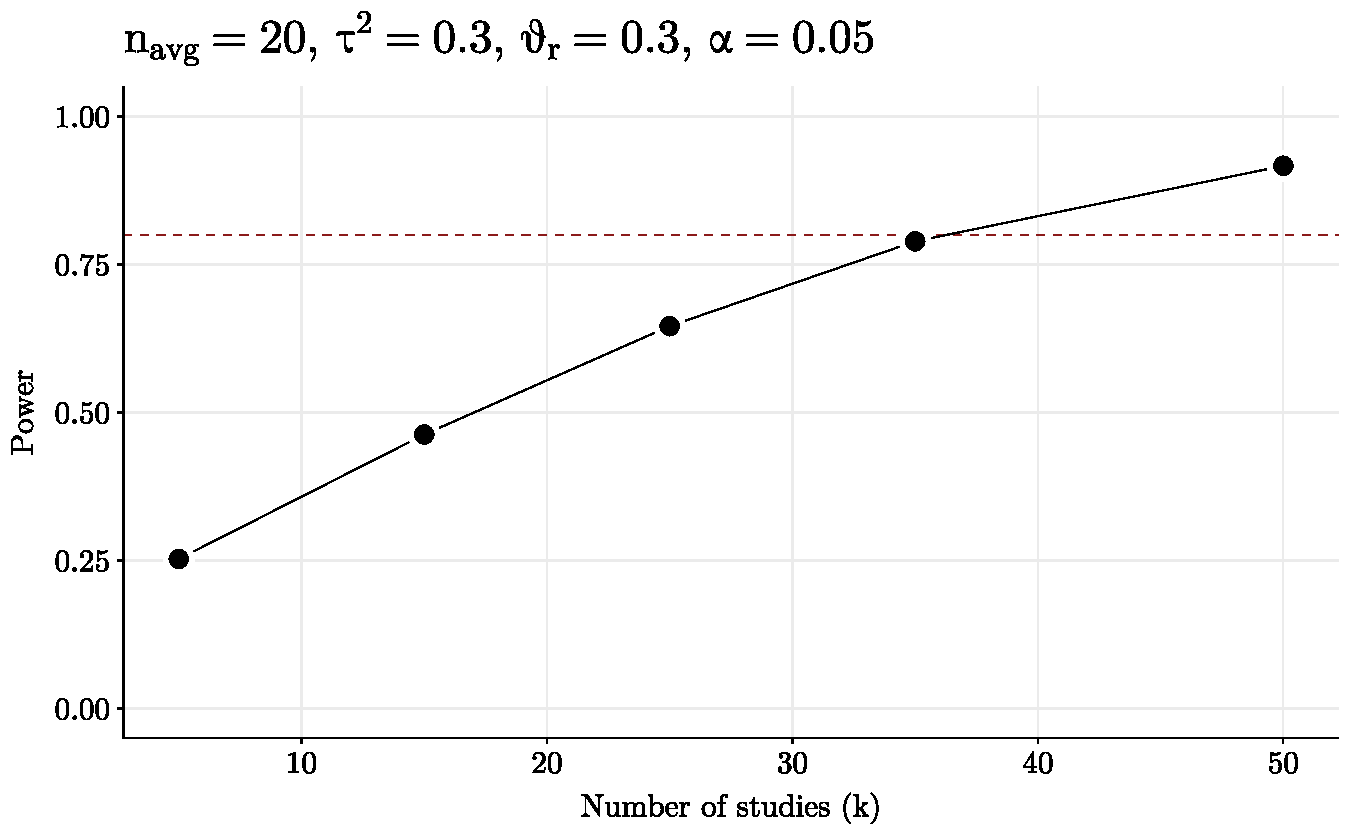
\includegraphics[width=0.8\linewidth]{paper_files/figure-latex/plot-power-analysis-1} 

}

\caption{Results from the \emph{random-effects model} power analysis. The x-axis depicts the number of studies (\(k\)), and the y-axis the estimated power. The red dotted line is the 80\% power level, usually considered a good value for power analysis.}\label{fig:plot-power-analysis}
\end{figure}

\normalsize

\hypertarget{conclusions}{%
\section{Conclusions}\label{conclusions}}

The present work introduced the basic concepts of the meta-analysis regarding fixed, random-effects models and meta-regression with a simulation-based approach. We believe the presented examples can help implement alternative or more complex models. For example, the \texttt{sim\_study()} function can be easily modified to simulate another effect sizes index, such as a paired sample Cohen's \(d\) or a Pearson's
correlation. In addition, more complex models, such as \emph{multivariate} or \emph{multilevel} models, can be implemented following the same approach (see supplementary materials). For example, the \emph{three-level} model estimates another heterogeneity component representing the variability of multiple effect sizes in the same study. Similarly, the \emph{multivariate} model could include the correlation between multiple outcomes and the correlation between sampling errors.

The present work did have a few limitations. First, we only introduced basic concepts about meta-analysis and Monte Carlo simulations, while setting up complex simulations requires more knowledge and complexity of the simulation setup. We decided to give the foundations to understand meta-analyses with a simulation approach because more complex models are still based on the same principles. Second, there are limitations
concerning simulating participant-level data. We decided to simulate the meta-analysis dataset starting from the participants' level to maximize the flexibility and clearness of each step. The downside concerns the efficiency and scalability of the simulation setup. For large-scale simulations (e.g., many conditions, iterations, or complex models), simulating from aggregated statistics is probably more efficient (see
Heuvel et al., 2020 for an example) to improve the computation speed\footnote{see \url{https://www.jepusto.com/simulating-correlated-smds/} for a very clear example of the participant-level vs aggregated data simulation}.

In conclusion, data simulation is a very powerful tool for each step of a data analysis process. Starting from the learning phase, where simulating data can be used to understand the statistical model in terms of assumptions and the data generation process, to the estimation of statistical power. Moreover, we believe that data simulation as part of a standard research workflow could improve the overall research quality. Data simulation requires understanding the statistical model, setting appropriate and reasoned parameters, and realizing how the chosen analysis method behaves across different scenarios.

\newpage

\hypertarget{acknowledgments}{%
\subsubsection*{Acknowledgments}\label{acknowledgments}}
\addcontentsline{toc}{subsubsection}{Acknowledgments}

We thank the \href{https://stat.ethz.ch/mailman/listinfo/r-sig-meta-analysis}{R-sig-meta-analysis} mailing-list where suggestions and clarifications significantly improved our simulations approach and the R code.

\hypertarget{conflicts-of-interest}{%
\subsubsection*{Conflicts of Interest}\label{conflicts-of-interest}}
\addcontentsline{toc}{subsubsection}{Conflicts of Interest}

The author(s) declare that there were no conflicts of interest with respect to the authorship or the publication of this article.

\hypertarget{data-materials-and-online-resources}{%
\subsubsection*{Data, materials, and online resources}\label{data-materials-and-online-resources}}
\addcontentsline{toc}{subsubsection}{Data, materials, and online resources}

The code to reproduce simulations, figures and tables can be found on Open Science Framework (\url{https://osf.io/54djn/})

\hypertarget{supplemental-material}{%
\subsubsection*{Supplemental Material}\label{supplemental-material}}
\addcontentsline{toc}{subsubsection}{Supplemental Material}

\hypertarget{prior-versions}{%
\subsubsection*{Prior versions}\label{prior-versions}}
\addcontentsline{toc}{subsubsection}{Prior versions}

The manuscript preprint has been uploaded on PsyArXiv \url{https://psyarxiv.com/br6vy/}

\newpage

\hypertarget{references}{%
\section*{References}\label{references}}
\addcontentsline{toc}{section}{References}

\hypertarget{refs}{}
\begin{CSLReferences}{1}{0}
\leavevmode\vadjust pre{\hypertarget{ref-Borenstein2009-mo}{}}%
Borenstein, M., Hedges, L. V., Higgins, J. P. T., \& Rothstein, H. R. (2009). \emph{Introduction to {Meta-Analysis}}. \url{https://doi.org/10.1002/9780470743386}

\leavevmode\vadjust pre{\hypertarget{ref-Cheung2014-fg}{}}%
Cheung, M. W.-L. (2014). Modeling dependent effect sizes with three-level meta-analyses: A structural equation modeling approach. \emph{Psychol. Methods}, \emph{19}(2), 211--229. \url{https://doi.org/10.1037/a0032968}

\leavevmode\vadjust pre{\hypertarget{ref-Cheung2015-bw}{}}%
Cheung, M. W.-L. (2015). \emph{{Meta-Analysis}: A structural equation modeling approach}. John Wiley \& Sons.

\leavevmode\vadjust pre{\hypertarget{ref-Cheung2019-po}{}}%
Cheung, M. W.-L. (2019). A guide to conducting a {Meta-Analysis} with {Non-Independent} effect sizes. \emph{Neuropsychol. Rev.}, \emph{29}(4), 387--396. \url{https://doi.org/10.1007/s11065-019-09415-6}

\leavevmode\vadjust pre{\hypertarget{ref-Cohen1988-ad}{}}%
Cohen, J. (1988). \emph{Statistical power analysis for the behavioral sciences} (2nd ed.). Routledge. \url{https://doi.org/10.4324/9780203771587}

\leavevmode\vadjust pre{\hypertarget{ref-DeBruine2021-id}{}}%
DeBruine, L. M., \& Barr, D. J. (2021). Understanding {Mixed-Effects} models through data simulation. \emph{Advances in Methods and Practices in Psychological Science}, \emph{4}(1), 2515245920965119. \url{https://doi.org/10.1177/2515245920965119}

\leavevmode\vadjust pre{\hypertarget{ref-Gelman2006-pc}{}}%
Gelman, A., \& Hill, J. (2006). \emph{Data analysis using regression and {Multilevel/Hierarchical} models}. Cambridge University Press. \url{https://doi.org/10.1017/CBO9780511790942}

\leavevmode\vadjust pre{\hypertarget{ref-Gelman2020-tg}{}}%
Gelman, A., Hill, J., \& Vehtari, A. (2020). \emph{Regression and other stories}. Cambridge University Press. \url{https://doi.org/10.1017/9781139161879}

\leavevmode\vadjust pre{\hypertarget{ref-Gentle2009-cj}{}}%
Gentle, J. E. (2009). Monte carlo methods for statistical inference. In J. E. Gentle (Ed.), \emph{Computational statistics} (pp. 417--433). New York, NY: Springer New York. \url{https://doi.org/10.1007/978-0-387-98144-4/_11}

\leavevmode\vadjust pre{\hypertarget{ref-Harrer2019-rl}{}}%
Harrer, M., Cuijpers, P., \& Ebert, D. (2019). \emph{Doing {Meta-Analysis} in {R}}. \url{https://doi.org/10.5281/zenodo.2551803}

\leavevmode\vadjust pre{\hypertarget{ref-Harrer2021-bz}{}}%
Harrer, M., Cuijpers, P., Furukawa, T. A., \& Ebert, D. D. (2021). \emph{Doing {Meta-Analysis} with r: A {Hands-On} guide}. CRC Press.

\leavevmode\vadjust pre{\hypertarget{ref-Hedges1981-za}{}}%
Hedges, L. V. (1981). Distribution theory for glass's estimator of effect size and related estimators. \emph{J. Educ. Behav. Stat.}, \emph{6}(2), 107--128. \url{https://doi.org/10.3102/10769986006002107}

\leavevmode\vadjust pre{\hypertarget{ref-Higgins2002-fh}{}}%
Higgins, J. P. T., \& Thompson, S. G. (2002). Quantifying heterogeneity in a meta-analysis. \emph{Stat. Med.}, \emph{21}(11), 1539--1558. \url{https://doi.org/10.1002/sim.1186}

\leavevmode\vadjust pre{\hypertarget{ref-Ingalls2011-xt}{}}%
Ingalls, R. G. (2011). Introduction to simulation. \emph{Proceedings of the 2011 Winter Simulation Conference ({WSC})}, 1374--1388. ieeexplore.ieee.org. \url{https://doi.org/10.1109/WSC.2011.6147858}

\leavevmode\vadjust pre{\hypertarget{ref-Jackson2017-dv}{}}%
Jackson, D., \& Turner, R. (2017). Power analysis for random-effects meta-analysis. \emph{Res. Synth. Methods}, \emph{8}(3), 290--302. \url{https://doi.org/10.1002/jrsm.1240}

\leavevmode\vadjust pre{\hypertarget{ref-Lakens2013-eq}{}}%
Lakens, D. (2013). Calculating and reporting effect sizes to facilitate cumulative science: A practical primer for t-tests and {ANOVAs}. \emph{Front. Psychol.}, \emph{4}, 863. \url{https://doi.org/10.3389/fpsyg.2013.00863}

\leavevmode\vadjust pre{\hypertarget{ref-Lipsey2001-vp}{}}%
Lipsey, M. W., \& Wilson, D. B. (2001). Practical meta-analysis. \emph{Applied Social Research Methods Series; Vol 49.}, \emph{247}.

\leavevmode\vadjust pre{\hypertarget{ref-Lopez-Lopez2014-it}{}}%
López-López, J. A., Marı́n-Martı́nez, F., Sánchez-Meca, J., Van den Noortgate, W., \& Viechtbauer, W. (2014). Estimation of the predictive power of the model in mixed-effects meta-regression: A simulation study. \emph{Br. J. Math. Stat. Psychol.}, \emph{67}(1), 30--48. \url{https://doi.org/10.1111/bmsp.12002}

\leavevmode\vadjust pre{\hypertarget{ref-r-lang}{}}%
R Core Team. (2022). \emph{R: A language and environment for statistical computing}. Vienna, Austria: R Foundation for Statistical Computing.

\leavevmode\vadjust pre{\hypertarget{ref-Schad2020-ht}{}}%
Schad, D. J., Vasishth, S., Hohenstein, S., \& Kliegl, R. (2020). How to capitalize on a priori contrasts in linear (mixed) models: A tutorial. \emph{J. Mem. Lang.}, \emph{110}, 104038. \url{https://doi.org/10.1016/j.jml.2019.104038}

\leavevmode\vadjust pre{\hypertarget{ref-Schmid2022-xe}{}}%
Schmid, C. H., Stijnen, T., \& White, I. R. (2022). \emph{Handbook of {Meta-Analysis}}. Taylor \& Francis Limited.

\leavevmode\vadjust pre{\hypertarget{ref-Viechtbauer2010-xz}{}}%
Viechtbauer, W. (2010). Conducting meta-analyses in {R} with the {metafor} package. \url{https://doi.org/10.18637/jss.v036.i03}

\end{CSLReferences}








































\end{document}
